\documentclass[11pt, oneside]{article}
\usepackage[utf8]{inputenc}
\usepackage{graphicx}
\usepackage[english, slovene]{babel}
\usepackage[autostyle]{csquotes}
\usepackage[a4paper, width=160mm, top=25mm, bottom=25mm]{geometry}

\usepackage{caption}
\usepackage{subcaption}

\usepackage{amsmath, amssymb, bm}

\usepackage{url}
\usepackage[dvipsnames, table]{xcolor}
\usepackage{hyperref}

\usepackage[stable]{footmisc}

\usepackage{booktabs}

\bibliographystyle{abbrv}
\usepackage[sorting=none]{biblatex}
\addbibresource{ref.bib}

\usepackage{amsthm}
\theoremstyle{definition}
\newtheorem{definition}{Definicija}

\newtheorem{theorem}{Izrek}

\graphicspath{{images/}}

\hypersetup{colorlinks=true, urlcolor=blue, linkcolor=blue, citecolor=blue}

\addto{\captionsslovene}{\renewcommand{\abstractname}{Besedilo naloge:}}

\begin{document}

\pagenumbering{gobble}

\begin{titlepage}
    \begin{center}
        \vspace*{0.8cm}

        \includegraphics[width=0.5\textwidth]{../../fmf_logo.png}
        \vspace{2cm}

        \large
        Modelska analiza

        \vspace{0.2cm}

        \Large
        \textbf{Zaključna naloga}

        \vspace{1cm}

        \normalsize
        Avtor: Jan Gavranovič \\
        \vspace{0.5cm}
        Predavatelj: prof. dr. Simon Širca \\
        Asistent: doc. dr. Miha Mihovilovič

        \vspace{0.5cm}

        avgust 2021

        \vspace{5cm}

        \begin{abstract}
            \noindent
            Preizkusi, ali lahko konkretne podatke uporabiš kot vir naključnih števil. Uporabiš lahko
            fizikalne meritve, geografske podatke (velikost mest, jezer, rek), zadnje objave na Twitterju ipd.
            Številske podatke moraš verjetno najprej transformirati, da dobiš bolj enakomerno porazdelitev.
            Namig: fizikalne  meritve  imajo  običajno  normalno  porazdeljen šum. Če se podatki raztezajo čez
            več velikostnih redov, Benfordov zakon trdi, da je običajno enakomerno porazdeljen logaritem vrednosti
            oz. vsaj njegov neceli del.
        \end{abstract}

    \end{center}
\end{titlepage}

\pagenumbering{arabic}

\tableofcontents

\vspace*{3cm}

\begin{figure}[h!]
    \centering
    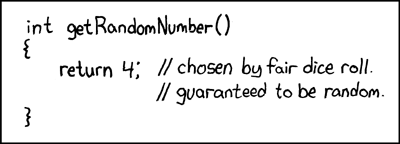
\includegraphics[width=0.6\textwidth]{random_number_xkcd.png}
    \caption{Generator ne preveč naključnih števil \cite{xkcd}.}
    \label{fig: 0}
\end{figure}

\newpage

\section{Psevdonaključna števila}
V numeričnih in statističnih postopkih pogosto potrebujemo števila, ki so čim bolj naključna.
Največkrat jih, v fiziki, potrebujemo za različne Monte Carlo simulacije, poleg tega pa se veliko uporabljajo tudi
v kriptografiji, kjer je kriteriji za naključnost precej strožji, kot pa pri simulacijah.
Računalnik sam od sebe ne more ustvariti pravih naključnih števil, zato uporabljamo deterministične generatorje
psevdonaključnih števil (PRNG). Skoraj v vseh primerih želimo imeti generator enakomerno porazdeljenih števil $U(0, 1)$, saj
lahko nato naredimo pretvorbo v števila porazdeljena po poljubni porazdelitvi.
Od dobrega enakomernega naključnega generatorja zaporedja $\{ x_i \}_{i=1}^N$ pričakujemo, da bo imel naslednje lastnosti \cite{sirca_verjetnost}:
\begin{itemize}
    \item Nekoreliranost zaporedja (podzaporedja $\{ x_i \}_{i=n}^{i+k}$ so čim manj korelirana, za vse $k$).
    \item Dolgo periodo zaporedja (čim dlje se ne sme ponoviti).
    \item Enakomernost in nepristranskost zaporedja (enako število točk pade v enako velik prostor).
    \item Serijsko enakomernost zaporedja (enakomerna porazdelitev točk $\{ x_i \}_{i=n}^{i+k-1}$ v hiperkocki s čim večjo dimenzijo $k$).
\end{itemize}

\subsection{Linearni kongruenčni generator}
Preden se lotimo naloge si naprej poglejmo nekaj determinističnih generatorjev,
ki jih bomo uporabili za primerjavo z generatorji pravih naključnih števil (TRNG).
Najbolj enostaven je linearni kongruenčni generator, ki je definiran z zvezo
\begin{equation}
    \label{eq: lkg}
    x_i = (ax_{i-1} + c) \text{ mod } m \>, \quad 0 \leq x_i < m \>,
\end{equation}
kjer je $a$ multiplikator, $c$ prirastek (\emph{increment}) in $m$ modulo generatorja.
Začetni vrednosti $x_0$ pravimo seme (\emph{seed}) generatorja. Rekurzivna zveza \ref{eq: lkg} nam vrne zaporedje
števil $\{ x_i \}$, ki jih lahko skaliramo, $u_i=x_i/m$, da dobimo enakomerno porazdelitev.
Vrednost $x_i$ določa vrednost $x_{i-1}$ in ker imamo samo $m$ različnih vrednosti, je perioda takega
generatorja enaka $m-1$ (ne štejemo $x_{i-1}=0$). Generator ima poleg tega še nekaj drugih težav
(vrednosti se zbirajo vzdolž hiperravnin), je pa zelo hiter in enostaven, zato se ga včasih še vedno uporablja.

\subsection{Mersenne Twister}
Sestavimo generator iz zaporedja bitov 0 in 1 z relacijo
\begin{equation}
    b_i = (a_p b_{i-p} + a_{p-1}b_{i-p+1} + \ldots + a_1 b_{i-1}) \text{ mod } 2 \>,
\end{equation}
kjer vse spremenljivke zavzamejo vrednosti 0 ali 1.
Vsota binarnih 0 in 1 z modulom 2 je enaka binarni exclusive-or operaciji $\oplus$.
Včasih se zgornje zapiše tudi z
\begin{equation}
    b_i = b_{i-p} \oplus b_{i-p+q} \quad \text{ali} \quad x_i = x_{i-p} \oplus x_{i-p+q} \>\> \text{ po bitih} \>.
\end{equation}
Algoritem se izvede kot \emph{feedback shift register}. Imamo vektor bitov, ki ga zamikamo za en bit levo. Zamaknjeni
bit po premiku kombiniramo z notranjim bitom z $\oplus$ in ga po operaciji dodamo na desni konec vektorja.
Slika \ref{fig: twotap} prikazuje opisan postopek, kjer kot vir bitov uporabimo dva vektorja (\emph{two tap}).
Algoritem Mersenne Twister deluje na osnovi množenja $x_{i-p+q}$ z matriko $A$:
\begin{equation}
    x_i = x_{i-p} \oplus A x_{i-p+q} \>.
\end{equation}
Vektorje bitov tako popačimo (\emph{twist}) z $A$ pred logičnim kombiniranjem, kar poveča naključnost $x_i$.
Perioda takega generatorja je $2^{19937}-1$. Algoritem je dober za generacijo naključnih števil
pri simulacijah, za kriptografske namene pa je neprimeren.

\newpage

\begin{figure}[h!]
    \centering
    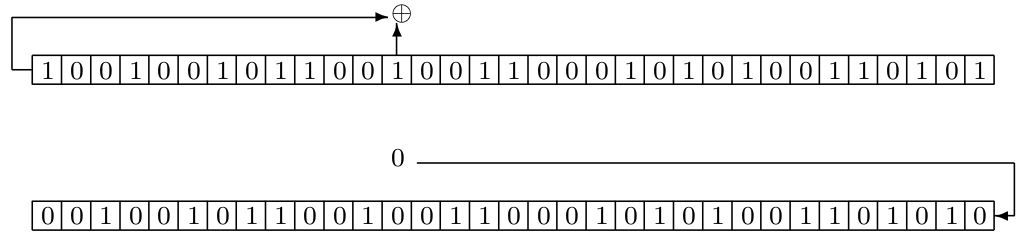
\includegraphics[width=0.82\textwidth]{two_tap.png}
    \caption{Primer zamikanja bitov v registru \cite{gentle2003random}.}
    \label{fig: twotap}
\end{figure}

Zanimivo si je pogledati še kako računalnik generira naključna števila, ki so potrebna za generacijo
raznih kriptografsko varnih ključev (SSL, SSH). Generatorja najdemo v \texttt{dev/random} in \texttt{dev/urandom}
na Linux sistemih \cite{arch}. Oba uporabljata algoritem ChaCha20, ki spada pod CSPRNG
(\emph{Cryptographically-secure PRNG}).
Razlika med njima je v tem, da \texttt{dev/random} uporabi tudi razne procese iz okolja, kot so vmesni časi
prekinitev, napak, odzivi tipkovnice in miške.

\section{Resnično naključna števila}
Radi bi generirali zares naključna števila. V ta namen rabimo podatke, ki izhajajo iz naključnega
procesa.
Primer takega procesa je radioaktivni razpad nestabilnega atomskega jedra, ki je zares naključen.
Verjetnost za razpad v nekem časovnem intervalu je odvisna samo od dolžine tega intervala.
Ob začetku merjenja je verjentost, da jedro ni razpadlo 1, potem pa eksponentno pada proti 0.
Za generacijo naključnega števila bi lahko uporabili dolžine časovnih intervalov $t_1$ in $t_2$
med dvema razpadoma, ki so tudi naključni. Če je $t_1 < t_2$, to pomeni bit 0, če je $t_1 > t_2$ pa bit 1,
kar nam na koncu da naključno zaporedje bitov.

Pri nalogi bom namesto idealnega (zgoraj opisanega) generatorja naključnih števil poskusil
uporabiti različne podatkovne sete. Od takega generatorja bom zahteval enake lastnosti, kot so bile opisane
za psevdonaključni generator. Prednost takega generatorja je, da nima periode in ne uporablja začetnega semena za
inicializacijo zaporedja. Največja slabost takega pristopa je količina naključnih števil (odvisna od
velikosti in kvalitete podatkovnega seta) ter počasna generacija, če ne uporabimo že izračunanih
in tabeliranih naključnih števil. Preden se lotimo iskanja podatkov in računaja naključnih števil si
poglejmo nekaj ključnih konceptov, ki nam bodo pri tem pomagali.

\section{Benfordov zakon}
Benfordov zakon, poznan tudi pod imenom zakon o anomalnih številih in zakon prve števke, je empirična
ugotovitev o porazdelitvi frekvenc vodilnih števk v izmerjenih numeričnih podatkih.
Zakon pravi, da vodilne števke številk v podatkih niso porazdeljene enakomerno, ampak so razporejene
padajoče. Benfordov zakon drži za različne tipe naravnih pojavov (cene delnic, računi za elektriko, matematične in fizikalne konstante itd.).
Zakon je podoben ugotovitvi, da  so po normalni (Gaussovi) porazdelitvi ali vsaj približno v skladu z njo porazdeljene številne količine
(telesne mase ljudi, izpitne ocene, hitrosti plinskih molekul itd.).
Zakon je najbolj točen, ko so vrednosti porazdeljene čez več velikostnih redov.
% in še posebaj, če je proces generacije številk posledica potenčnega zakona $f(x)=ax^{-k}$, torej za porazdelitve z dolgimi repi.

Benfordov zakon drži za množico številk, če se vodilne števke $d \in \{1, 2,\ldots,9 \}$ pojavijo z
verjetnostmi
\begin{equation}
    \label{eq: benford}
    P(d) = \log_{10} (d+1) - \log_{10}(d)  = \log_{10} \left ( 1 + \frac{1}{d} \right ) \>.
\end{equation}
Zgornja enačba je zapisana v desetiški bazi, zakon pa velja tudi v vseh ostalih in ni posledica izbire številskega sistema.
Količina $P(d)$ je odvisna od razdalje med števko $d+1$ in $d$ v logaritemski skali.
% , torej je to pričakovana porazdelitev, če so logaritmi števil porazdeljeni enakomerno in naključno.

\newpage

Imejmo število $x \in \{1, 10\}$, ki se začne z 1, če $1 \leq x < 2$ ali z 2, če $2 \leq x < 3$ in tako naprej do števila 10.
V logaritemski skali se število začne z 1, če $\log 1 \leq \log x < \log 2$ ali z 2, če $\log 2 \leq \log x < \log 3$ in tako naprej do števila 10.
Vidimo, da so zaporedni intervali v logaritemski skali vse ožji ($|\log 1 - \log 2| \approx 0.301$, $|\log 2 - \log 3| \approx 0.176$, $\ldots$, $|\log 9 - \log 10| \approx 0.046$),
kot je prikazano v spodnji tabeli.

\begin{table}[h!]
    \begin{center}
        \begin{tabular}{|c|c|c|c|c|c|c|c|c|c|}
            \hline$d$    & 1        & 2        & 3        & 4        & 5        & 6        & 7        & 8        & 9        \\
            \hline$P(d)$ & $0.3010$ & $0.1761$ & $0.1249$ & $0.0969$ & $0.0792$ & $0.0669$ & $0.0580$ & $0.0512$ & $0.0458$ \\
            \hline
        \end{tabular}
    \end{center}
    \caption{Verjetnosti za prvo števko po Benfordovem zakonu.}
    \label{tab: 1}
\end{table}

% Če je torej $\log x$ enakomerno porazdeljen, potem je bolj verjetno, da se številka začne z manjšo števko.
% Verjetnosti so odvisne od razlike zaporednih števk po zgornji formuli.
% Bolj strogo lahko tudi zahtevamo, da morajo biti enakomerno porazdeljeni ne celi deli logaritma števila.

Naj bo $\{ x_i\}_{i=1}^N$ zaporedje realnih števil iz enakomerne porazdelitve vzorčeno na intervalu
$x_i\in [p \log_a 10,\> (p+1) \log_a 10)$, kjer je $p$ poljubno celo število (npr. $p=0$).
Potem se porazdelitev prve (ali katerikoli druge) števke zaporedja $\{ a^{x_i} \}_{i=1}^N$ približuje
Benfordovemu zakonu pri $N \rightarrow \infty$. V logaritemski skali je verjetnost, da $\log_a a^{x_i}$ pade v
razred $b_d$ sorazmerna s širino tega razreda deljeno s širino celotnega intervala
\begin{equation}
    P(\log_a a^{x_i} \in b_d) = \frac{\log_a \left ( (d+1) \cdot 10^p \right ) - \log_a \left ( d \cdot 10^p \right ) }{\log_a 10^{p+1} - \log_a 10^p} = \frac{\log_a \frac{1+d}{d}}{\log_a 10} = \log_{10} \left ( 1 + \frac{1}{d} \right ) \>,
\end{equation}
kar nam da nazaj Benfordov zakon \cite{romerorochin2009derivation}.
V nadaljevanju bomo videli, da obstaja močnejša različica Benforodvega zakona, ki vključuje necele dele
števila, kar nam bo prišlo bolj prav, saj podatki ponavadi nimajo oblike $\{ a^{x_i} \}_{i=1}^N$.

Zanimivo je tudi odkritje Benfordovega zakona. Prvi je pojav zapisal kanadsko-ameriški astronom Simon Newcomb
leta 1881. Pri uporabi logaritemskih tabel je opazil, da so začetne strani (na začetku so vrednosti, ki se začnejo z 1)
veliko bolj obrabljene kot pa vse ostale. Svoja opažanja je skupaj s formulacijo zakona objavil v
kratkem članku na dveh straneh \cite{newcomb}. Pojav je ponovno odkril ameriški fizik Frank Benford leta 1938 in ga tudi bolj
podrobno dokumentiral. Za preizkus je med drugim uporabil površine rek, velikosti mest, hišne številke znanih ljudi,
fizikalne konstante in molekulske mase.

V primeru, da je porazdelitev prve števke invariantna na skaliranje s poljubno konstanto (neodvisna od enot v kateri
so zapisani podatki), potem je porazdelitev prvih števk podana z Benfordovim zakonom.
Če torej podatki sledijo Benfodovemu zakonu, potem je delež prve števke (in vseh ostalih) vedno približno konstanten pri zaporednem
množenju s konstanto.

\subsection{Matematične in fizikalne konstante}
Za začetek preizkusimo Benfordov zakon na matematičnih in fizikalnih konstantah.
Uporabil sem 464 konstant iz \cite{scipy_const}. Pojavitve prvih števk so prikazane na grafu \ref{fig: ben_konst}.
Vidimo, da prve števke konstant precej dobro sledijo Benfordovemu zakonu.
Porazdelitev logaritma konstant je prikazana na sliki \ref{fig: ben_konst1} in ni enakomerna.
Na sliki \ref{fig: ben_konst2} je prikazana še porazdelitev necelega dela logaritma konstant, ki pa je
približno enakomerna. Invariantnost na skaliranje sem preveril z zaporednim množenjem z 1.01, kar
prikazuje slika \ref{fig: ben_konst3}. Dobljena odvisnost je periodična, saj se prva števka začne ponavljati
pri takem množenju. Vidimo, da je delež enic niha okrog povprečja, ki je okrog 0.3, ki ga tudi napove
Benfordov zakone. Amplituda oscilacij okrog te ravnovesne vrednosti pove, kako dobro podatki sledijo
Benfordovemu zakonu.

Podobna ugotovitev velja za količine, ki jih je preučeval že Benford (pregled je v \cite{scott2001benford}).
Problem je, da imamo pri takih podatkih na voljo bolj malo števil (okrog $\mathcal{O}(10^3)$), ki jih potem
uporabimo za pretvorbo v naključna števila.

\newpage

\vspace*{0.5cm}

\begin{figure}[h!]
    \centering
    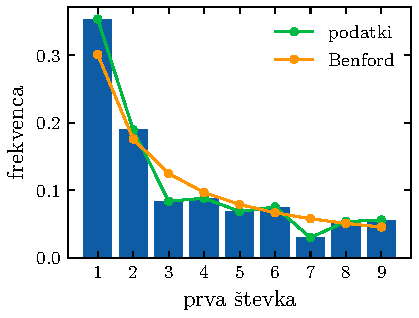
\includegraphics[width=0.45\textwidth]{benford_konstante_prva_stevka.pdf}
    \caption{Delež prvih števk v konstantah. Z oranžno je prikazana odvisnost \ref{eq: benford}.}
    \label{fig: ben_konst}
\end{figure}

\begin{figure}[h!]
    \centering
    \begin{subfigure}[b]{0.49\textwidth}
        \centering
        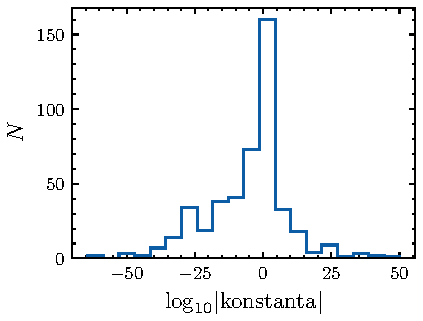
\includegraphics[width=0.9\textwidth]{benford_konstante_log.pdf}
        \caption{Logaritem konstant.}
        \label{fig: ben_konst1}
    \end{subfigure}
    \hfill
    \begin{subfigure}[b]{0.49\textwidth}
        \centering
        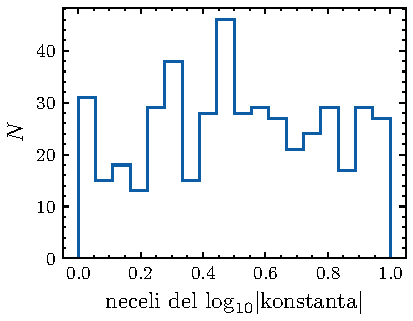
\includegraphics[width=0.88\textwidth]{benford_konstante_neceli.pdf}
        \caption{Neceli del logaritma konstant.}
        \label{fig: ben_konst2}
    \end{subfigure}
    \caption{Porazdelitev vrednosti matematičnih in fizikalnih konstant.}
\end{figure}

\begin{figure}[h!]
    \centering
    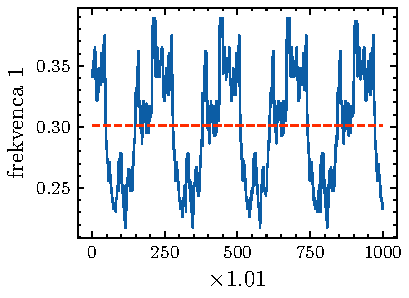
\includegraphics[width=0.45\textwidth]{benford_konstante_freq_1.pdf}
    \caption{Invariantnost na skaliranje s konstanto.}
    \label{fig: ben_konst3}
\end{figure}

\newpage
\subsection{Spektralna analiza Benfordovega zakona}
Radi bi vedeli kdaj bo porazdelitev sledila Benfordovemu zakonu. Slika \ref{fig: ben_konst3} že namiguje na uporabo
spektralne analize \cite{10.5555/281875}. Za bolj sistematičen opis si za testno funkcijo (signal) izberemo lognormalno
porazdelitev z verjetnostno gostoto
\begin{equation}
    \label{eq: lognormal}
    f_X(x) = \frac{1}{x \sigma \sqrt{2\pi}} \exp{\left ( -\frac{(\log x - \mu)^2}{2\sigma^2} \right ) }
\end{equation}
s parametroma $\sigma$ in $\mu$, ki predstavljata pričakovano vrednost in standardno deviacijo logaritma spremenljivke
$X$. Če je naključna spremenljivka $X$ lognormalno porazdeljena, potem je $Y=\ln X$ normalno porazdeljena.
Osnova logaritma pri tem ni pomembna, če je $\log_a(X)$ normalno porazdeljen, potem je tudi $\log_b(X)$ za vse
pozitivne $a, b\neq 1$.
Uporaba te porazdelitve je prikladna za Benfordov zakon, saj že vemo, da se morajo podatki raztezati čez
več velikostnih redov, da zakon drži. Na sliki \ref{fig: lognorm1} so prikazane tri različno široke
lognormalne porazdelitve, ki so normirane v logaritemski skali. Preostali grafi prikazujejo deleže enic pri skaliranju s konstanto.

\begin{figure}[h!]
    \centering
    \begin{subfigure}[b]{0.49\textwidth}
        \centering
        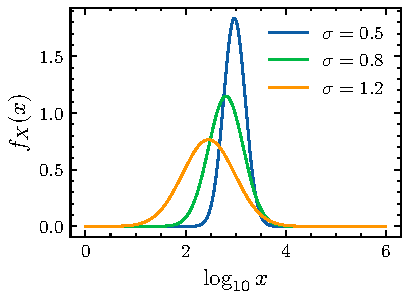
\includegraphics[width=0.9\textwidth]{lognormal_dist.pdf}
        \caption{Različne lognormalne porazdelitve.}
        \label{fig: lognorm1}
    \end{subfigure}
    \hfill
    \begin{subfigure}[b]{0.49\textwidth}
        \centering
        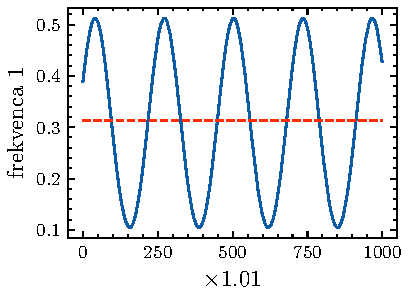
\includegraphics[width=0.9\textwidth]{benford_lognorm_freq_1_mu05.pdf}
        \caption{$\sigma=0.5$.}
        \label{fig: lognorm2}
    \end{subfigure}
    \hfill
    \begin{subfigure}[b]{0.49\textwidth}
        \centering
        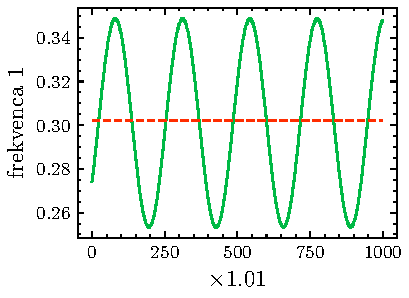
\includegraphics[width=0.9\textwidth]{benford_lognorm_freq_1_mu08.pdf}
        \caption{$\sigma=0.8$.}
        \label{fig: lognorm3}
    \end{subfigure}
    \hfill
    \begin{subfigure}[b]{0.49\textwidth}
        \centering
        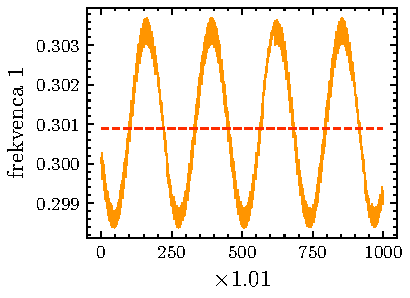
\includegraphics[width=0.9\textwidth]{benford_lognorm_freq_1_mu12.pdf}
        \caption{$\sigma=1.2$.}
        \label{fig: lognorm4}
    \end{subfigure}
    \caption{Lognormalne porazdelitve, ki različno dobro sledijo Benfordovemu zakonu.}
    \label{fig: lognorm}
\end{figure}

\noindent
Do števila enic v številkah podatkov lahko pridemo na več načinov. Najbolj enostaven je algoritem pri katerem
množimo ali delimo številko z 10 dokler ni to število med $\geq1$ in $<10$ ter na koncu preštejemo vse
enice (slike \ref{fig: lognorm}).
Ta postopek spremeni številke glede na potence števila 10, ki nam potem da logaritemski vzorec Benfordovega zakona.

Izpeljimo sedaj ekvivalenten postopek štetja enic s pomočjo Fourierove transformacije.
Sestavimo vzorčevalno funkcijo $s$ (\emph{sampling function}), ki je enaka 1 v območju kjer se
število začne z 1 in 0 drugje (slika \ref{fig: sf}). Vrednosti porazdelitve $f$, ki se začnejo z 1 dobimo z
množenjem $s \cdot f$. Delež enic dobimo z integracijo produkta
\begin{equation}
    n_1(g) = \int_{-\infty}^{\infty} s(g) f(g) dg \>,
\end{equation}
kjer $g$ označuje logaritemsko skalo. Invariantnost na skaliranje preverimo z večkratnim računanjem
\begin{equation}
    n_1(k) = \int_{-\infty}^{\infty} s(g) f(g - k) dg \>,
\end{equation}
kjer je $k$ konstanten premik, ki je v logaritemski skali zaporedno seštevanje z neko majhno konstanto, npr. $\log f +\log1.01$.
Izpeljali smo postopek, ki nam vrne verjetnost, da se številka iz porazdelitve $f$ začne z 1 za poljuben skalirni
faktor $k$. Krajše lahko postopek zapišemo kot konvolucijo v logaritemski skali
\begin{equation}
    n_1(g) = s(g) * f(g) \>.
\end{equation}
Prestavimo se v frekvenčni prostor v katerem se konvolucija zapiše kot produkt transformirank
\begin{equation}
    \mathcal {F}\left [ n_1(g) \right ] = \mathcal{F} [s(g)] \cdot \mathcal{F} [f(g)] \> \Rightarrow \>
    n_1(g) = \mathcal{F}^{-1} \left \{ \mathcal{F} [s(g)] \cdot \mathcal{F} [f(g)] \right \} \>.
\end{equation}
Opisan postopek je prikazan na sliki \ref{fig: FFT}. Vrednost pri 0 v frekvenčnem prostoru vedno ustreza povprečni
vrednosti signala. Tako je ničta (DC) komponenta transformiranke porazdelitve vedno 1, saj je porazdelitev normirana.
Ničta komponenta transformiranke vzorčevalne funkcije in s tem tudi ničta komponenta konvolucije pa je
enaka povprečnemu deležu enic v porazdelitvi (povprečju signala iz slike \ref{fig: e}).
Povprečni delež enic (slika \ref{fig: e}) je za vse tri porazdelitve enak, saj je
ničta komponenta konvolucije neodvisna od porazdelitve, kar je posledica tega, da je porazdelitev normirana
(ničta komponenta $\mathcal{F}[s]$ se množi z 1).

Končno lahko tudi odgovorimo na začetno vprašanje, ali bo dana porazdelitev sledila Benfordovemu zakonu ali pa mu ne bo.
Želimo imeti tako porazdelitev $f$, ki bo vrnila konstanto vrednost $n_1=0.301$ za vse premike $k$.
Povprečje $n_1$ je vedno 0.301 ne glede na to ali podatki sledijo Benfordovemu zakonu ali pa mu ne.
Pomembne so torej oscilacije okrog povprečja. $n_1$ torej ne sme imeti nobenih sinusoidnih komponent.
V frekvenčnem prostoru to pomeni, da mora biti konvolucija $\mathcal{F} [s(g)] \cdot \mathcal{F} [f(g)]$ enaka 0
pri frekvencah višjih od 0. Vemo tudi, da je $\mathcal{F}[s(g)]$ neničelna samo pri celoštevilskih
frekvencah $f=0,1,2,\ldots$ iz česar izpeljemo, da bo $n_1$ konstanta samo, če bo vrednost
porazdelitve v frekvenčnem prostoru $\mathcal{F} [f(g)]$ enaka nič za vse cele frekvence $f=1,2,3$ in tako naprej.

Vrnimo se nazaj k sliki \ref{fig: lognorm1}. Odgovor na to zakaj prvi dve ($\sigma=0.5$ in $\sigma=0.8$)
porazdelitvi ne sledita Benfordovemu zakonu je v njihovi širini. Če je porazdelitev ozka, potem bo njena
Fourierova transoformiranka široka in obratno. Široka porazdelitev v frekvenčnem prostoru
pomeni veliko neničelno komponento pri $f=1$, kar nakazuje na prisotnost sinusnih nihanj pri izračunu
konvolucije, kar po inverzni Fourierovi transformaciji vidimo kot oscilacije okrog povprečnega deleža enic.

Na sliki \ref{fig: lognorm_sigma} je prikazana odvisnost Fourierove komponente porazdelitve pri frekvenci 1 od
parametra širine porazdelitve $\sigma$. 

\vspace*{-0.2cm}

\begin{figure}[h!]
    \centering
    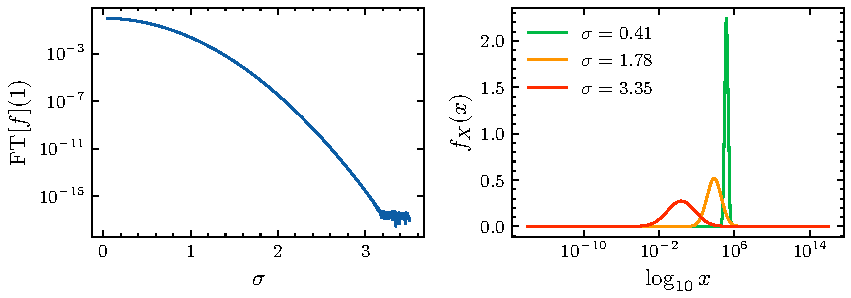
\includegraphics[width=0.9\textwidth]{sigma_FT.pdf}
    \caption{Benfordov zakon in širina porazdelitve.}
    \label{fig: lognorm_sigma}
\end{figure}

\newpage

\vspace*{1cm}

\begin{figure}[h!]
    \centering
    \begin{subfigure}[b]{0.49\textwidth}
        \centering
        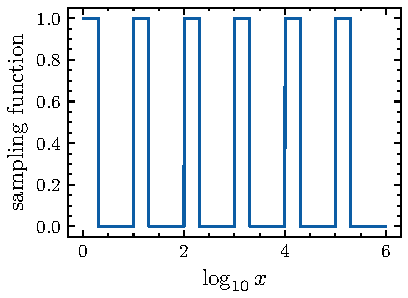
\includegraphics[width=0.88\textwidth]{lognorm_sampling_function.pdf}
        \caption{Vzorčevalna funkcija.}
        \label{fig: sf}
    \end{subfigure}
    \hfill
    \begin{subfigure}[b]{0.49\textwidth}
        \centering
        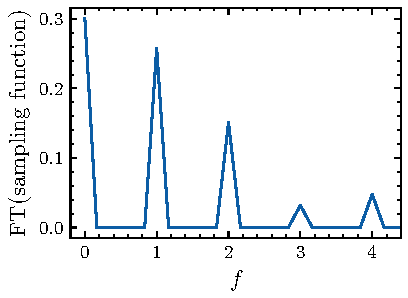
\includegraphics[width=0.9\textwidth]{lognorm_FT_sampling_function.pdf}
        \caption{$\mathcal{F}[s(g)]$.}
    \end{subfigure}
    \hfill
    \begin{subfigure}[b]{0.49\textwidth}
        \centering
        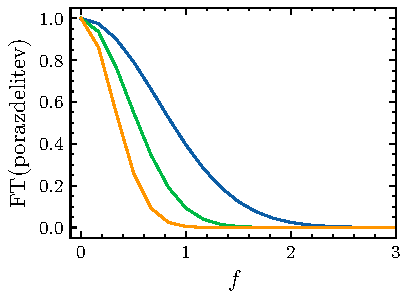
\includegraphics[width=0.9\textwidth]{lognorm_FT_pdf.pdf}
        \caption{$\mathcal{F}[f(g)]$.}
    \end{subfigure}
    \hfill
    \begin{subfigure}[b]{0.49\textwidth}
        \centering
        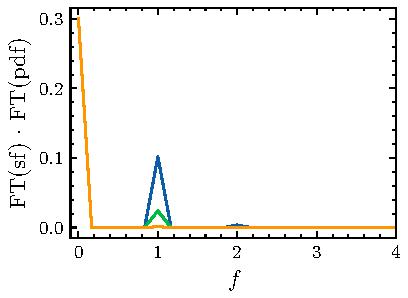
\includegraphics[width=0.9\textwidth]{lognorm_conv.pdf}
        \caption{$\mathcal{F}[s(g)] \cdot \mathcal{F}[f(g)]$.}
    \end{subfigure}
    \hfill
    \begin{subfigure}[b]{0.49\textwidth}
        \centering
        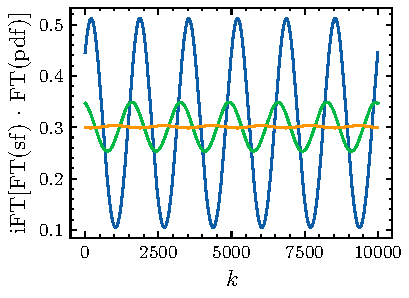
\includegraphics[width=0.9\textwidth]{lognorm_ost.pdf}
        \caption{$\mathcal{F}^{-1} \left \{ \mathcal{F} [s(g)] \cdot \mathcal{F} [f(g)] \right \}$.}
        \label{fig: e}
    \end{subfigure}
    \caption{Vzorčevalna funkcija in njena Fourierova transformiranka, Fourierova transformacija lognormalne porazdelitve,
        konvolucija v frekvenčnem prostoru in prikaz verjetnosti, da se številka iz lognormalne porazdelitve začne z 1.}
    \label{fig: FFT}
\end{figure}

\newpage
\section{Statistični testi za enakomerno porazdelitev} % \footnote{Delno povzeto po \cite{sirca_verjetnost}.}
Benfordov zakon nam pove, da so neceli deli logaritma števila porazdeljeni približno po enakomerni porazdelitvi.
Enakomernost take porazdelitve je seveda odvisna od tega kako dobro podatki sledijo Benfordovemu zakonu.
Kriterij za sledenje Benfordovemu zakonu smo že našli v velikosti prve neničelne frekvenčne komponente
Fourierove transformiranke verjetnostne gostote. Poleg tega bi radi imeli še dodaten kriterij, ki nam bo povedal
kako ``dobra'' je dobljena enakomerna porazdelitev, oziroma, če je porazdelitev sploh skladna z enakomerno. Čim bolj bo porazdelitev enakomerna, tem boljši bo
generator naključnih števil narejen iz podatkov te porazdelitve.

\subsection{Pearsonov test $\chi^2$}
Imamo množico $n$ podatkov (izmerkov), ki jih razvrstimo v $N$ razredov (\emph{binov}).
% Preizkušamo hipotezo $H_0: f(x) = f_0(x)$, kjer je $f_0$ verjetnostna gostota ali verjetnostna funkcija. 
V $i$-tem razredu pričakujemo $f_i$ dogodkov, dejansko pa se jih v njem nahaja $n_i$.
Ničelna hipoteza je
\begin{equation}
    H_0: f_1=f_{01},f_2=f_{02}, \ldots, f_N=f_{0N} \>,
\end{equation}
testna statistika pa je
\begin{equation}
    \chi^2 = \sum_{i=1}^N \frac{(n_i - f_{0i})^2}{f_{0i}} \>.
\end{equation}
Če hipoteza $H_0$ velja, je $\chi^2$ porazdeljena po porazdelitvi $\chi^2$ z $N-p$ prostostnimi stopnjami, kjer je $p$ število
parametrov, ki so bili ocenjeni iz vzorca. V primeru, da je ničelna hipoteza enakomerna porazdelitev, je pričakovano število
dogodkov v vsakem razredu
\begin{equation}
    f_{0i} = \frac{N}{n} \>.
\end{equation}
Hipotezo $H_0:f_\text{izmerjena}=f_\text{enakomerna}$ na koncu preverimo ob neki stopnji zaupanja $1-\alpha$.

\subsection{Test Kolmogorov-Smirnova (KS)}
Je neparametrični test s katerim primerjamo vzorec z modelsko porazdelitvijo, ali pa primerjamo dva vzorca med seboj.
Pove ali vzorec izvira iz populacije, porazdeljene v skladu s teoretično modelsko porazdelitvijo, ali da en
vzorec izvira iz enake populacije kot drugi. Izmerjene vrednosti $\{ x_i \}_{i=1}^n$ razvrstimo po velikosti
in definiramo empirično porazdelitveno funkcijo
\begin{equation}
    \label{eq: KS_F}
    \widetilde{F}_n(x) =
    \begin{cases}
         & 0 \>;\> x < x_1 \>,                                           \\
         & i/n \>;\> x_i \leq x < x_{i+1} \>, \quad i=1,2,\ldots,n-1 \>, \\
         & 1 \>;\> x \geq x_n \>,                                        \\
    \end{cases}
\end{equation}
ki je monotona naraščajoča, stopničasta funkcija. Test primerja empirično porazdelitveno funkcijo $\widetilde{F}_n$
z modelsko porazdelitveno funkcijo $F$. Ničelna hipoteza je tako
\begin{equation}
    H_0: \widetilde{F}_n(x)=F(x) \>,
\end{equation}
kjer bomo za modelsko porazdelitveno funkcijo uporabili
\begin{equation}
    F(x) =
    \begin{cases}
         & 0 \>;\hfill x < 1 \>,                                   \\
         & \frac{x - a}{b - a} \>;\quad \hfill a \leq x \leq b \>, \\
         & 1 \>;\hfill x > b \>.                                   \\
    \end{cases}
\end{equation}
Testna statistika pa je maksimalna razdalja med porazdelitvama
\begin{equation}
    D_n = \underset{x}{\text{sup}} \left | \widetilde{F}_n(x) - F(x) \right | \>,
\end{equation}
kjer je porazdelitev statistike $D_n$ je znana in je neodvisna od porazdelitve $F$.

\newpage

\subsection{Enakomerna porazdelitev in Benfordov zakon}
Označimo z $\langle x \rangle$ neceli del realnega števila $x$, ki ga dobimo kot
\begin{equation}
    \langle x \rangle = x - \lfloor x \rfloor \>, \quad x > 0 \>,
\end{equation}
kjer $\lfloor \cdot \rfloor$ predstavlja največje celo število manjše ali enako realnemu številu $x$ (\emph{floor function}).
Enakomerno porazdelitev bomo sestavili s pomočjo naslednjega teorema (formalna matematična obravnava z dokazi je zapisana v \cite{berger2011basic}):
\begin{theorem}
    Zaporedje $\{x_1, x_2, \ldots, x_N \}$ realnih števil je Benfordovo natanko tedaj, ko je neceli del logaritma
    absolutne vrednosti enakomerno porazdeljen.
\end{theorem}
\noindent
Neko zaporedje števil $\{x_i \}_{i=1}^N$ je torej Benfordovo, če je zaporedje
$\{ \langle \log_{10}|x_i| \rangle \}_{i=1}^N$ enakomerno porazdeljeno. Z drugimi besedami, zaporedje je Benfordovo,
če je logaritem absolutne vrednosti tega zaporedja porazdeljen enakomerno modulo 1.

Zapišimo logaritem števila kot vsoto celega dela (karakteristike) in necelega dela (mantise):
\begin{equation}
    \log_{10} x_i = C(x_i) + m(x_i) \>.
\end{equation}
Antilogaritmiranje nam vrne $10^{\log_{10}x_i}=10^{C(x_i)} 10^{m(x_i)}$. Vidimo, da $10^{C(x_i)}$ pove položaj
decimalne vejice in $10^{m(x_i)}$ dejanske številke, zato je porazdelitev števil odvisna samo od necelega
dela $m(x_i)$. Če so torej neceli deli zaporedja $\{ m(x_i) \}_{i=1}^N$ enakomerno porazdeljeni, potem so enakomerno porazdeljeni tudi
$\{ 10^{m(x_i)} \}_{i=1}^N$ in s tem tudi $\{ x_i \}_{i=1}^N$.

Vrnimo se za trenutek nazaj k lognormalni porazdelitvi \ref{eq: lognormal}.
Zmnožek $n$ pozitivnih naključnih spremenljivk nam da, v limiti $n \rightarrow \infty$, približno
lognormalno porazdelitev. Ugotovitev sledi iz centralnega limitnega izreka.
Podobno nam centralni limitni izrek pove, da seštevanje naključnih spremenljivk vodi do normalne
porazdelitve, ki pa ne sledi Benfordovemu zakonu.
Poglejmo si še povezavo med normalno in lognormalno porazdelitvijo.
Povezava med parametri je \cite{enwiki:1034516769}:
\begin{equation}
    \mu = \ln \left ( \frac{\mu_X^2}{\sqrt{\mu_X^2 + \sigma_X^2}} \right ) \quad \text{in} \quad
    \sigma^2 = \ln \left ( 1 + \frac{\sigma_X^2}{\mu_X^2}  \right ) \>,
\end{equation}
kjer sta $\mu$ in $\sigma^2$ povprečje in varianca normalne porazdelitve ter $\mu_X$ in $\sigma^2_X$ ekvivalentna
parametra lognormalne porazdelitve. Formuli bomo uporabili za lažjo predstavo o tem, kako široka je lognormalna
porazdelitev ($\sigma$ pove širino lognormalne porazdelitve v logaritemski skali, ki jo obravnavamo kot normalno).

Na sliki \ref{fig: lognorm_uni} so prikazane porazdelitve necelega dela logaritma za lognormalne porazdelitve z
različnim parametrom $\sigma$. Porazdelitve sem generiral po \ref{eq: lognormal} z uporabo vgrajenega generatorja
naključnih števil. Na slikah so zapisane tudi vrednosti testnih statistik, na zadnji sliki pa so še
kritične vrednosti $\chi^2_*$ in $d_*$ pri $\alpha=0.01$.
Samo za zadnjo porazdelitev lahko trdimo, da je skladna z enakomerno s stopnjo zaupanja $99\%$.

Vrednosti obeh testov v odvisnosti od širine porazdelitve prikazuje slika \ref{fig: test1}.
Parameter $\sigma$ je podan za lognormalno porazdelitev in tudi kot ekvivalenten parameter normalne porazdelitve (zgornja skala).
Iz grafa vidimo, da moramo imeti lognormalno porazdelitev s $\sigma_X \gtrsim 1.5$,
da bo zadoščeno ničelni hipotezi o skladnosti z enakomerno porazdelitvijo na stopnji zaupanja $1-\alpha=0.99$.

Na sliki \ref{fig: test2} je prikazana odvisnost obeh vrednosti statistik v odvisnosti od prve Fourierove frekvenčne
komponente $f_1$. Zaradi končnega naključnega vzorca vrednost $f_1$ ne pada pod $10^{-4}$ kljub povečevanju
$\sigma$. Iz obeh grafov vidimo, da bomo morali za dobro naključno generacijo števil poiskati proces, ki bo
vrnil podatke porazdeljene po lognormalni porazdelitvi široki vsaj nekaj velikostnih redov.

% signifikand teorija 
% Signifikand realnega števila (včasih tudi mantisa) je njegov koeficient pri zapisu s floating-point (znanstveno) notacijo.
% Tako je signifikand števila $2021=2.021 \cdot 10^3$ enak 2.021. Formalna definicja signifikandne funkcije je \cite{berger2011basic}:
% \begin{definition}
%     Decimalna signifikandna funkcija $S: \mathbb{R} \rightarrow [1, 10)$ je definirana sledeče: če $x \neq 0$
%     potem je $S(x)=t$, kjer je $t$ iz $[1, 10)$ in za njega velja $|x|=10^k t$ za nek $k\in \mathbb{Z}$. Če je $x=0$, 
%     potem si izberemo $S(0):=0$.
% \end{definition}
% \noindent
% Eksplicitno je $S$ podana z 
% \begin{equation}
%     S(x) = 10^{\log_{10}|x| - \lfloor \log_{10} |x| \rfloor} \quad \text{za vse } x \neq 0 \>, 
% \end{equation}
% kjer $\lfloor \cdot \rfloor$ predstavlja največje celo število manjše ali enako realnemu številu $x$ (\emph{floor function}).
% Vidimo tudi, da za vse $x \in \mathbb{R}$ velja
% \begin{equation}
%     S(10^kx) = S(x) = S(S(x)) \quad \text{za vse } k \in \mathbb{Z} \>.
% \end{equation}

\newpage

\vspace*{0.45cm}

\begin{figure}[h!]
    \centering
    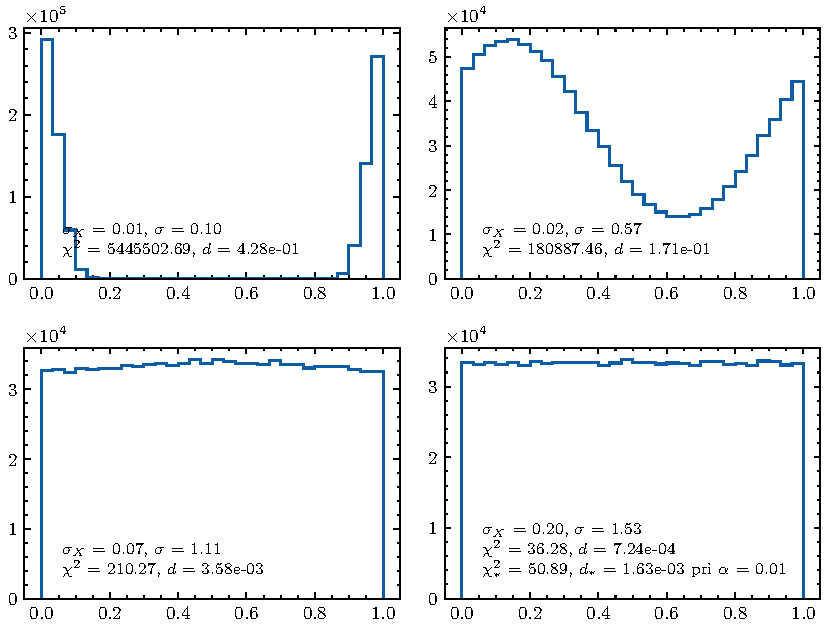
\includegraphics[width=0.85\textwidth]{lognorm_uniform_hists.pdf}
    \caption{Porazdelitve necelega dela logaritma naključnih števil žrebanih iz različnih lognormalnih porazdelitev.
        Na slikah so zapisani tudi rezultati opisanih statističnih testov.}
    \label{fig: lognorm_uni}
\end{figure}

\begin{figure}[h!]
    \centering
    \begin{subfigure}[b]{0.49\textwidth}
        \centering
        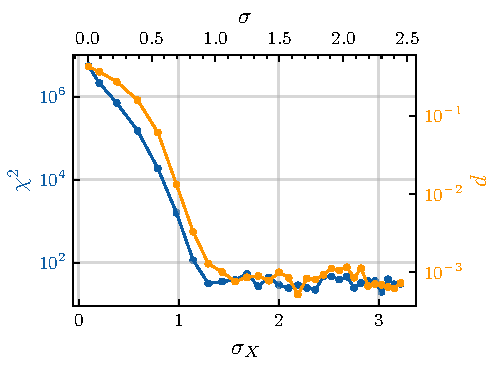
\includegraphics[width=1\textwidth]{stat_lognorm_tests.pdf}
        \caption{Vrednosti testa  $\chi^2$ in testa KS v odvisnosti od parametra $\sigma$ lognormalne porazdelitve in $\sigma_X$ normalne porazdelitve.}
        \label{fig: test1}
    \end{subfigure}
    \hfill
    \begin{subfigure}[b]{0.49\textwidth}
        \centering
        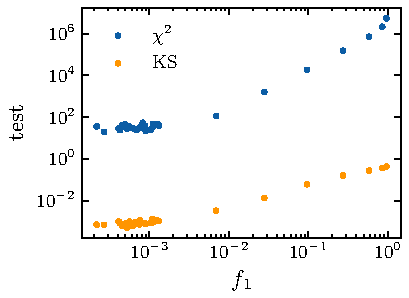
\includegraphics[width=0.9\textwidth]{test_lognorm_f1_chi2_KS.pdf}
        \caption{Odvisnost vrednosti testnih statistik od širine porazdelitve podane s prvo Fourierovo frekvenčno komponento.}
        \label{fig: test2}
    \end{subfigure}
    \caption{Prikaz različnih odvisnosti pri računanju enakomerne porazdelitve.}
    \label{fig: test}
\end{figure}

\newpage

\section{Kakovost generatorjev naključnih števil}
Kakovosti generatorjev naključnih števil preverjamo s statistično utemeljenimi baterijami empiričnih testov.
Za preverjanje kakovosti dobljenih naključnih števil sem uporabil zbirko NIST Statisical Test Suite,
poznano tudi pod imenom SP 800-22. Testi kot vhodni podatek vzamejo zaporedje naključnih
bitov ter vrnejo uspešnost testa (true/false) glede na $p$-vrednost pri $\alpha=0.01$ (s to verjetnostjo se test zmoti in vrne false namesto true, \emph{type I error}).
Naključno zaporedje bitov je sestavljeno iz 0 in 1, kjer so biti med seboj neodvisni in se pojavijo z verjetnostjo $1/2$.
Ničta hipoteza $H_0$ je, da je testirano zaporedje bitov naključno, alternativna hipoteza pa je, da zaporedje
ni naključno. Vseh testov je 15 in so podrobno opisani ter tudi implementirani v originalnem članku \cite{sp800-22},
zato jih bom tukaj samo navedel (tabela \ref{tab: 2}), jih bom pa uporabil za končno testiranje generatorja.
Najbolj pomemben je prvi (frekvenčni) test, ki preverja enakomerno porazdelitev bitov. Če odpove prvi, potem
je nadaljnje testiranje nesmiselno.
\begin{table}[h!]
    \begin{center}
        \begin{tabular}{c|c}
            \#              & ime testa                                      \\
            \hline \hline 1 & The Frequency (Monobit) Test                   \\
            \hline 2        & Frequency Test within a Block                  \\
            \hline 3        & The Runs Test                                  \\
            \hline 4        & Tests for the Longest-Run-of-Ones in a Block   \\
            \hline 5        & The Binary Matrix Rank Test                    \\
            \hline 6        & The Discrete Fourier Transform (Spectral) Test \\
            \hline 7        & The Non-overlapping Template Matching Test     \\
            \hline 8        & The Overlapping Template Matching Test         \\
            \hline 9        & Maurer's "Universal Statistical" Test          \\
            \hline 10       & The Linear Complexity Test                     \\
            \hline 11       & The Serial Test                                \\
            \hline 12       & The Approximate Entropy Test                   \\
            \hline 13       & The Cumulative Sums (Cusums) Test              \\
            \hline 14       & The Random Excursions Test                     \\
            \hline 15       & The Random Excursions Variant Test             \\
        \end{tabular}
    \end{center}
    \caption{Vrstni red in imena testov.}
    \label{tab: 2}
\end{table}

\section{Naključna števila iz fizikalnih podatkov}

\subsection{Življenjski čas miona}
Pri eksperimentu merimo življenjski čas mionov, ki nastanejo pri interakcijah visokoenergijskih kozmičnih
delcev z molekulami v zgornjih plasteh atmosfere. Mion ima dva glavna razpadna kanala
\begin{equation}
    \mu^+ \rightarrow e^+ + \nu_e + \overline{\nu}_\mu
\end{equation}
in
\begin{equation}
    \mu^- \rightarrow e^- + \overline{\nu}_e + \nu_\mu \>.
\end{equation}
Za detekcijo mionov smo uporabili sod z mineralnim oljem z dodatkom scintilatorja in fotopomnoževalko, ki je
delno potopljena vanj. Ko mion preleti sod povzroči scintilacije, ki jih zaznamo kot več-fotonski signal s
fotopomnoževalko. Mioni večinoma sod samo preletijo in se v njem ne ustavijo.
Če pa imajo dovolj nizko energijo, se v scintilatorju ustavijo in razpadejo.
Tako nastala elektron ali pozitron v scintilatorskem olju znova zasvetita, kar ponovno izmerimo.
Z meritvijo časa med nastankom obeh sunkov (slika \ref{fig: mu1}) lahko ugotovimo razpadni čas miona.

\newpage
Na slikah so prikazane meritve pri dveh različno dolgih časih merjenja, ki sem jih naredil pri
predmetu Fizikalni eksperimenti. Pri vsaki meritvi imamo na voljo $10^3$ podatkovnih točk iz
katerih bomo poskusili dobiti naključna števila. Na izmerjene podatke v logaritemski skali naprej prilagodimo
premico (slika \ref{fig: mu2}). Prilagojena premica predstavlja linearni trend, ki ga odštejemo od podatkov,
da dobimo normalno porazdeljen šum (slika \ref{fig: mu_noise}).

% https://en.wikipedia.org/wiki/Probability_integral_transform
% Dobljeno normalno porazdelitev lahko
% sedaj spremenimo v enakomerno preko integralske verjetnostne transformacije, ki pravi, da je naključna spremenljivka $Y$
% definirana kot komulativna verjetnostna funkcija $Y=F_X(x)$ zvezne naključne spremenlivke $X$ enakomerno porazdeljena.
% Izračunati moramo torej empirično porazdelitveno funkcijo, ki je enaka \ref{eq: KS_F} in je prikazana na sliki \ref{fig: ecdf}.
% Dobili smo preslikavo, ki slika vrednosti porazdelitve enakomerno na interval $(0, 1]$. Pri izračunu smo
% vrednosti v zaporedju meritev $\{ x_i \}_{i=1}^N$ razvrstili po velikosti. Za generacijo naključnih števil moramo
% dobljene vrednosti na intervalu $(0, 1]$ razvrstit nazaj v začetni vrstni red, da dobimo naključno zaporedje. Takšna generacija naključnih
% števil odpove, če imamo podatke že na začetku razvrščene v nekem vrstnem redu (v našem primeru
% obravnavamo šum in to ni pomembno).

% https://stats.stackexchange.com/questions/117689/simulating-draws-from-a-uniform-distribution-using-draws-from-a-normal-distribut
% https://www.google.com/search?channel=fs&client=ubuntu&q=any+distribution+to+unifrom
% https://en.wikipedia.org/wiki/Box%E2%80%93Muller_transform
Iz dobljene normalne porazdelitve bi radi naredili enakomerno porazdelitev.
Normalno porazdelitev najprej spremenimo v standardno normalno z uvedbo
\begin{equation}
    Z = \frac{X - \mu}{\sigma} \>,
\end{equation}
kjer parametra $\mu$ in $\sigma$ dobimo s fitom na podatke. Uporabili bomo obratno Box-Mullerjevo transformacijo.
Naj bosta $U_1$ in $U_2$ neodvisna vzorca iz enakomerne porazdelitve na intervalu $(0, 1)$.
Neodvisni naključni spremenljivki $Z_1$ in $Z_2$, porazdeljeni po standardni normalni porazdelitvi $N(0, 1)$, dobimo s
transformacijo
\begin{equation}
    Z_1 = R \cos \theta = \sqrt{-2 \ln U_1} \cos 2 \pi U_2 \quad \text{in} \quad
    Z_2 = R \sin \theta = \sqrt{-2 \ln U_1} \sin 2 \pi U_2 \>,
\end{equation}
kjer spremenljivki $U_1$ in $U_2$ določata dolžino in kot ravninskega vektorja $[Z_1, Z_2]^\top$
\begin{equation}
    R = \sqrt{-2 \ln U_1} \quad \text{in} \quad \theta = 2\pi U_2 \>.
\end{equation}
Z nekaj računanja dobimo obratni zvezi, ki povezujeta enakomerno porazdelitev s standardno normalno:
\begin{equation}
    U_1 = \exp\left[{- \frac{\left(Z_1^2 + Z_1 \sqrt{Z_1^2 + Z_2^2} + Z_2^2\right)^2}{2 \left(Z_1 + \sqrt{Z_1^2 + Z_2^2}\right)^2}} \right]
    \quad \text{in} \quad
    U_2 = - \frac{1}{\pi} \arctan \left( \frac{Z_1 + \sqrt{Z_1^2 + Z_2^2}}{Z_2} \right) \>.
\end{equation}
Tako dobljeni enakomerni porazdelitvi prikazuje slika \ref{fig: box_muller}. Pri $\alpha=0.01$ lahko rečemo, da je
prva enakomerna (druga je pa precej blizu).

Pojavi se še vprašanje kako dobiti zaporedje bitov iz zaporedje realnih števil (32 ali 64 bitni float v računalniku).
Lahko se sprehajamo po binarnem odločitvenem drevesu pri čemer tvorimo:
\begin{equation}
    \label{eq: decide}
    \text{odločitev} =
    \begin{cases}
         & \text{bit } 0 \>, \quad \text{če} \quad x_i \leq 0.5 \>, \\
         & \text{bit } 1 \>, \quad \text{če} \quad x_i > 0.5 \>,
    \end{cases}
\end{equation}
% bit 0, če $x_i \leq 0.5$ in bit 1, če $x_i > 0.5$,
kar nam da naključno zaporedje bitov (en bit za vsako naključno številko).
Druga možnost je, da direktno spremenimo število v binarno reprezenatacijo.
Pri tem se moramo zavedati IEEE 754 formata, ki je za 32 bitno število na sliki \ref{fig: float}.
Če želimo imeti naključno zaporedje bitov, moramo torej izpustiti prvih 9 bitov, ki predstavljajo
predznak in eksponent števila (imamo enakomerno porazdelitev zato se večina števil začne z 00111111).
Postopek nam iz enega naključnega števila da 23 bitov.

Tabela \ref{tab: 3} prikazuje uspešnost testov \ref{tab: 2} za generirana naključna števila iz obeh meritev.
Indeksa 1 in 2 se nanašata na prvo in drugo enakomerno porazdelitev $U_1$ in $U_2$.
Indeks 3 se nanaša na združeni porazdelitvi (v smislu bitnih zaporedij).
Za generacijo bitnega zaporedja sem uporabil drugi opisani postopek.
Spodleti samo test 12, ki preverja frekvence prekrivanja $m$-bitnega vzorca. Razlog za to je
verjetno prekratko zaporedje bitov, saj za združeno (daljše) zaporedje dobimo pozitiven rezultat.

Zaporedje bitov lahko predstavimo tudi v kvadratni matriki, kar prikazuje slika \ref{fig: m} za
prvo meritev. Na levi sliki je po diagonalah jasno opazen vzorec, ki se pojavi, če v zaporedju
vzamemo vseh 32 bitov (očitno ni naključen). Desna slika prikazuje naključen vzorec pri katerem upoštevamo bite, ki se
ne ponavljajo.

\newpage

% https://stackoverflow.com/questions/867602/quickest-way-to-generate-random-bits
\vspace*{-1cm}
\begin{figure}[h!]
    \centering
    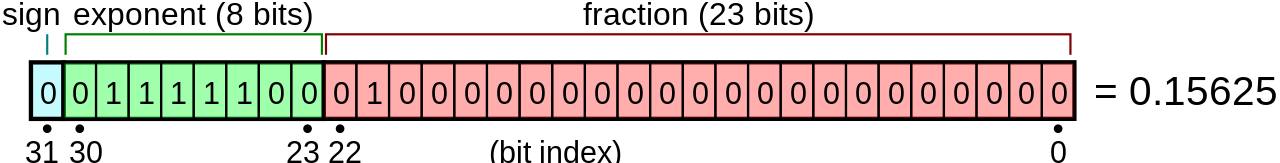
\includegraphics[width=0.7\textwidth]{float.png}
    \caption{Enojna natančnost binarnega števila \cite{enwiki:floats}.}
    \label{fig: float}
\end{figure}

\begin{figure}[h!]
    \centering
    \begin{subfigure}[b]{0.49\textwidth}
        \centering
        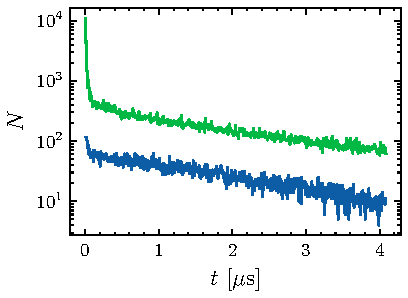
\includegraphics[width=0.9\textwidth]{mioni_meritve.pdf}
        \caption{Meritve.}
        \label{fig: mu1}
    \end{subfigure}
    \hfill
    \begin{subfigure}[b]{0.49\textwidth}
        \centering
        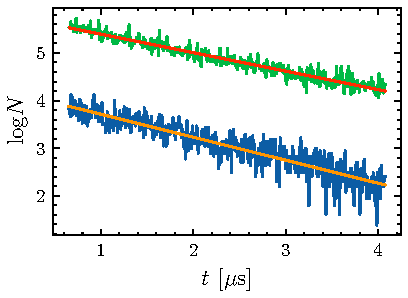
\includegraphics[width=0.9\textwidth]{mioni_fit.pdf}
        \caption{Linearni fit v logaritemski skali.}
        \label{fig: mu2}
    \end{subfigure}
    \caption{Meritev časa napetostnih sunkov in prilagajanje linearne odvisnosti.}
    \label{fig: mu}
\end{figure}

\begin{figure}[h!]
    \centering
    \begin{subfigure}[b]{0.49\textwidth}
        \centering
        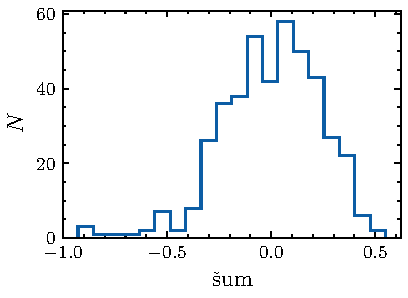
\includegraphics[width=0.9\textwidth]{mioni_sum_0.pdf}
        \label{fig: mu_noise1}
    \end{subfigure}
    \hfill
    \begin{subfigure}[b]{0.49\textwidth}
        \centering
        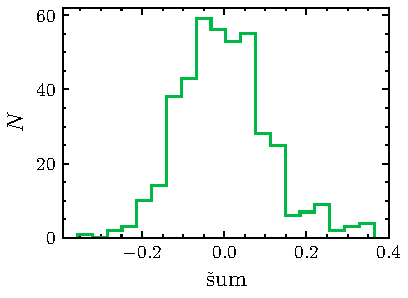
\includegraphics[width=0.9\textwidth]{mioni_sum_1.pdf}
        \label{fig:mu_noise2}
    \end{subfigure}
    \caption{Normalni šum obeh meritev, ki ga dobimo z odštevanjem linearnega trenda.}
    \label{fig: mu_noise}
\end{figure}


\begin{figure}[h!]
    \centering
    \begin{subfigure}[b]{0.49\textwidth}
        \centering
        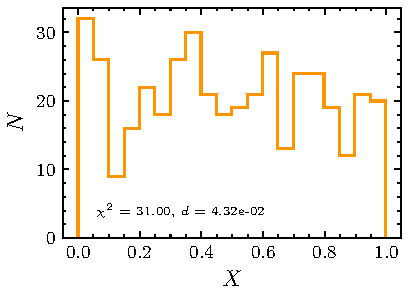
\includegraphics[width=0.9\textwidth]{box_muller_uniform_0.pdf}
    \end{subfigure}
    \hfill
    \begin{subfigure}[b]{0.49\textwidth}
        \centering
        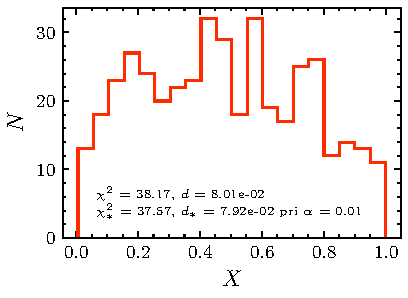
\includegraphics[width=0.9\textwidth]{box_muller_uniform_1.pdf}
    \end{subfigure}
    \caption{Enakomerni porazdelitvi generirani z obratno Box-Mullerjevo transformacijo.}
    \label{fig: box_muller}
\end{figure}

\newpage

\begin{table}[h!]
    \begin{center}
        \hspace*{-0.8cm}
        \begin{tabular}{cccccccccccccccc}
            \toprule
            {}    & 1    & 2    & 3    & 4    & 5    & 6    & 7    & 8    & 9   & 10   & 11   & 12                       & 13   & 14   & 15   \\
            \midrule
            $p_1$ & 0.40 & 0.27 & 0.62 & 0.64 & 0.21 & 0.07 & 0.31 & 0.91 & nan & 0.82 & 0.69 & \cellcolor{red!40} 0.00  & 0.72 & 0.67 & 0.59 \\
            $p_2$ & 0.38 & 0.14 & 0.32 & 0.35 & 0.13 & 0.43 & 0.81 & 0.28 & nan & 0.85 & 0.66 & \cellcolor{red!40}  0.00 & 0.37 & 0.33 & 0.82 \\
            \rowcolor{green!40}
            $p_3$ & 0.23 & 0.16 & 0.28 & 0.77 & 0.42 & 0.02 & 0.29 & 0.86 & nan & 0.68 & 0.73 & 0.02                     & 0.25 & 0.67 & 0.58 \\
            \bottomrule
        \end{tabular}
    \end{center}
    \caption{Rezultati statističnih testov za naključna števila iz šuma meritev. Vrednost \texttt{nan} pomeni premajhen vzorec za dani statistični test.}
    \label{tab: 3}
\end{table}

\begin{figure}[h!]
    \centering
    \begin{subfigure}[b]{0.49\textwidth}
        \centering
        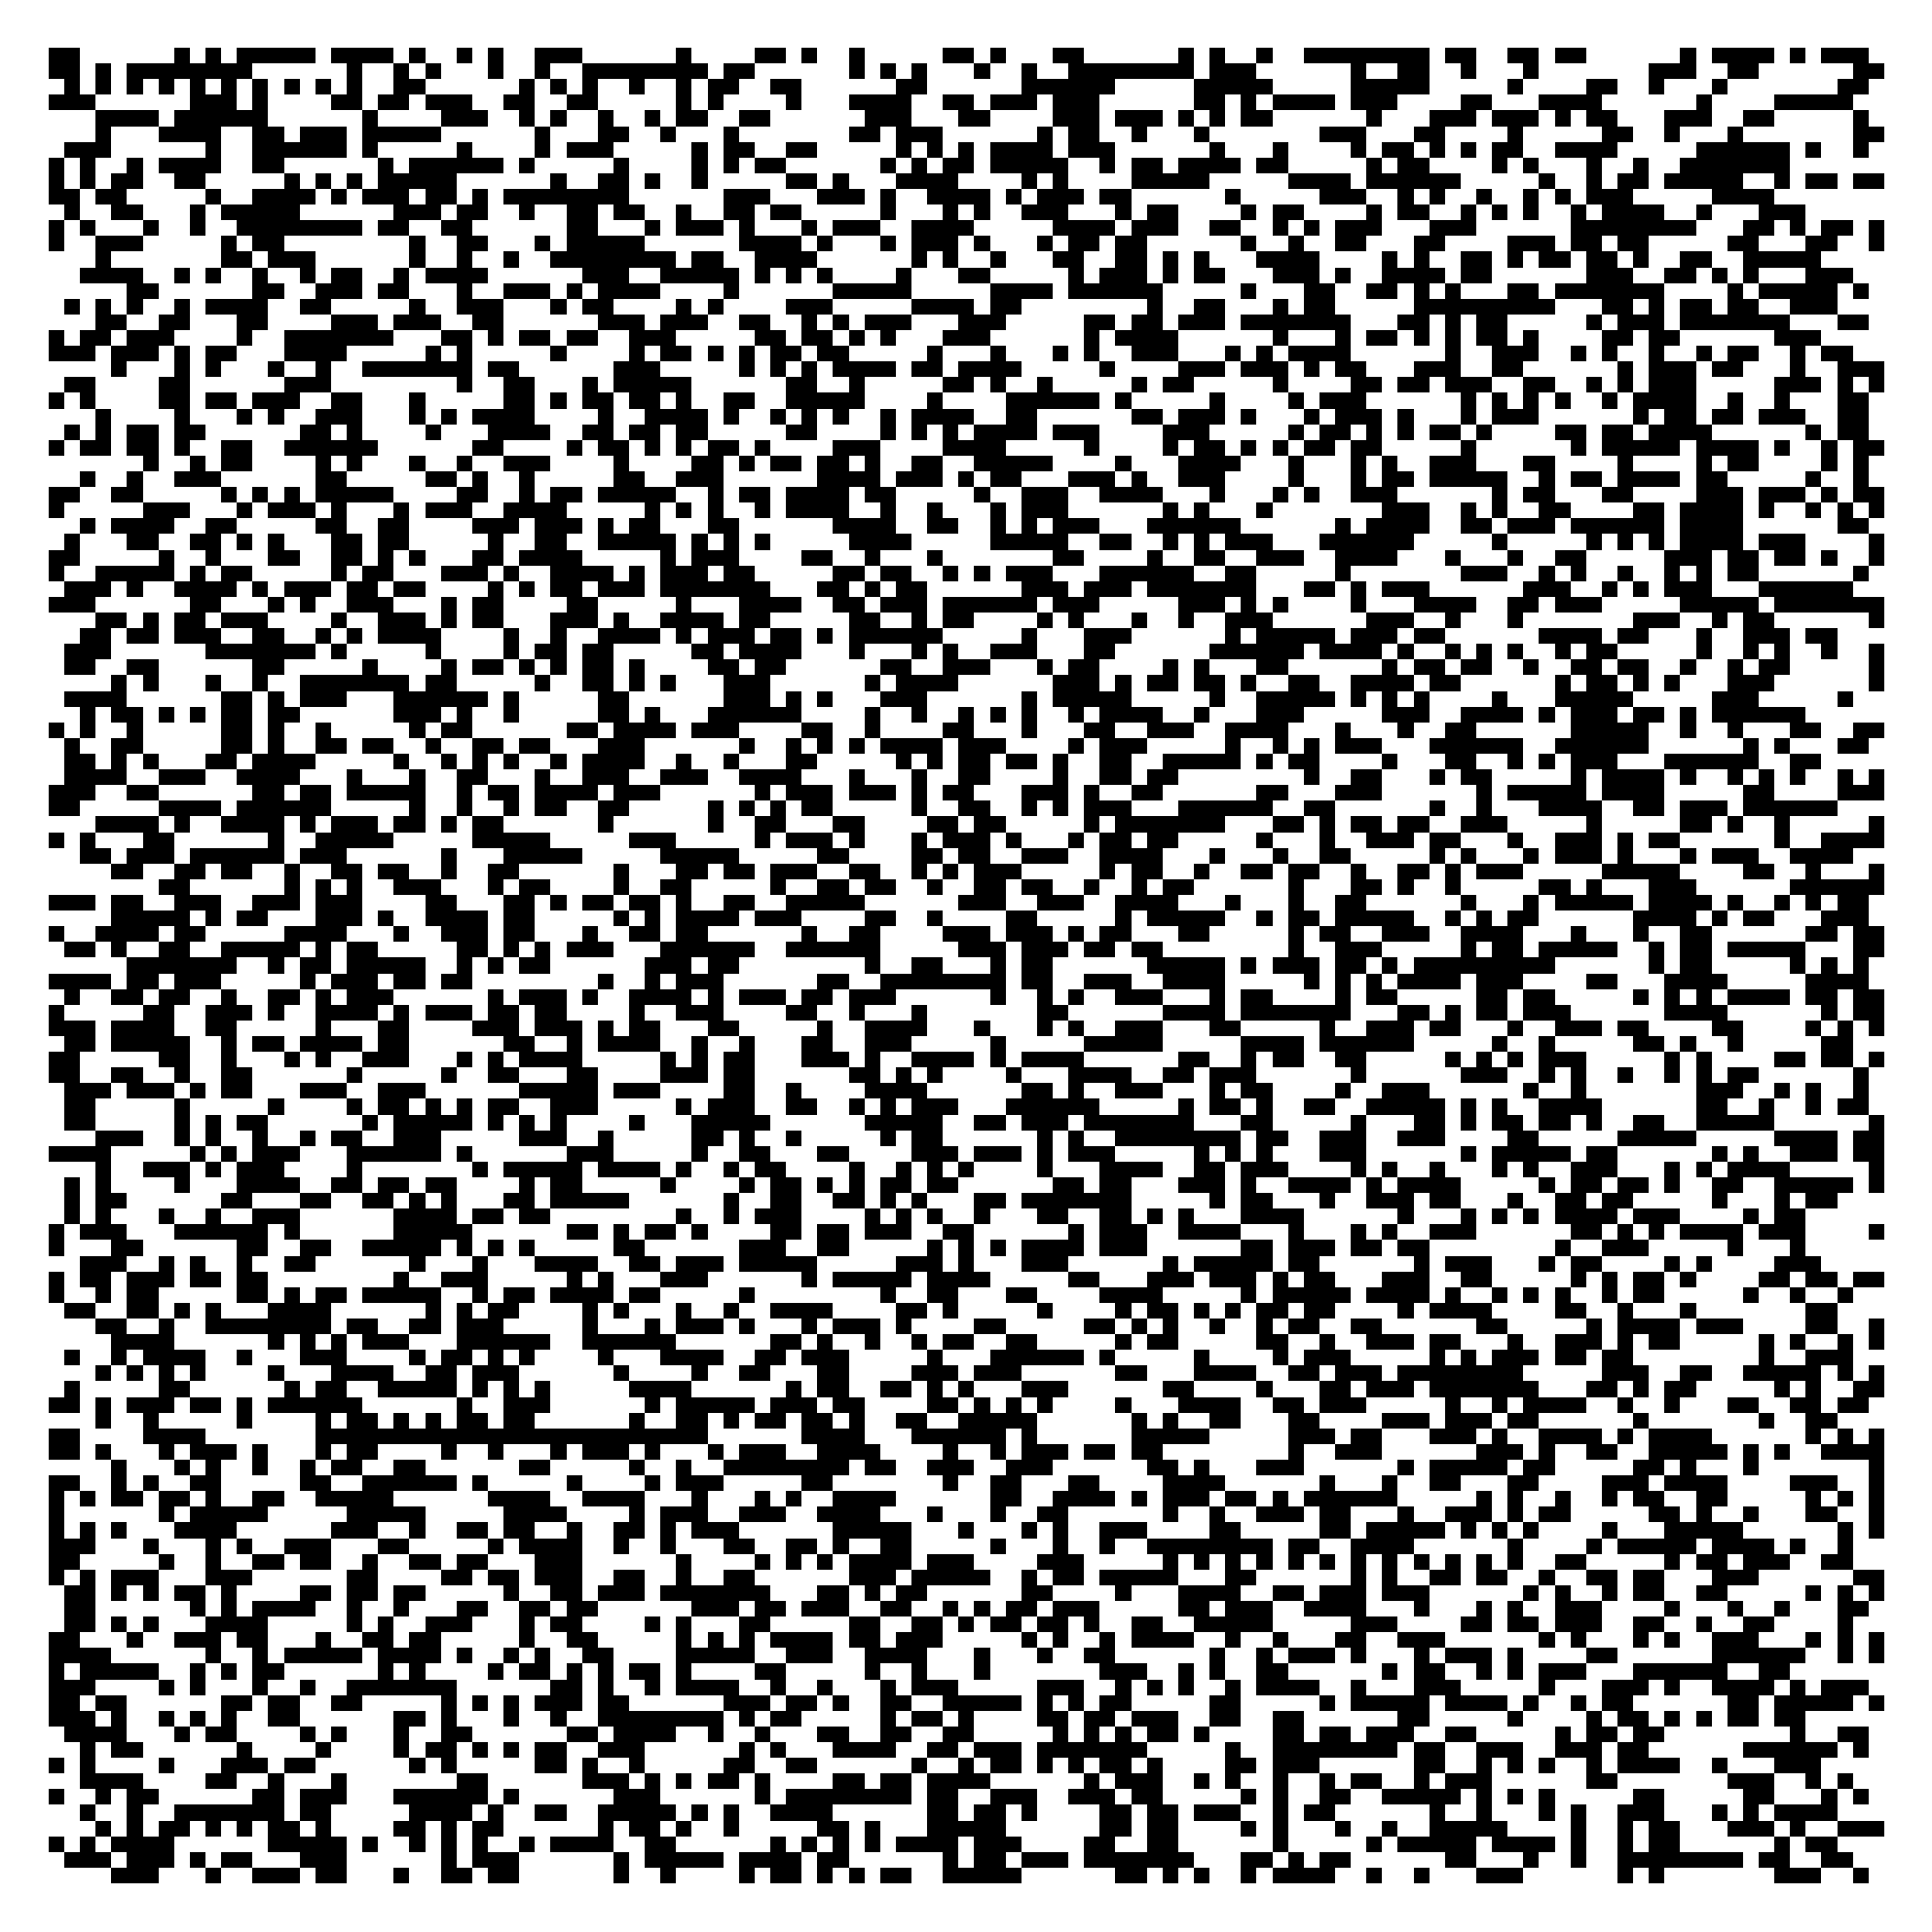
\includegraphics[width=0.7\textwidth]{mioni_matrika_slaba.png}
        \caption{}
        \label{fig: m1}
    \end{subfigure}
    \hfill
    \begin{subfigure}[b]{0.49\textwidth}
        \centering
        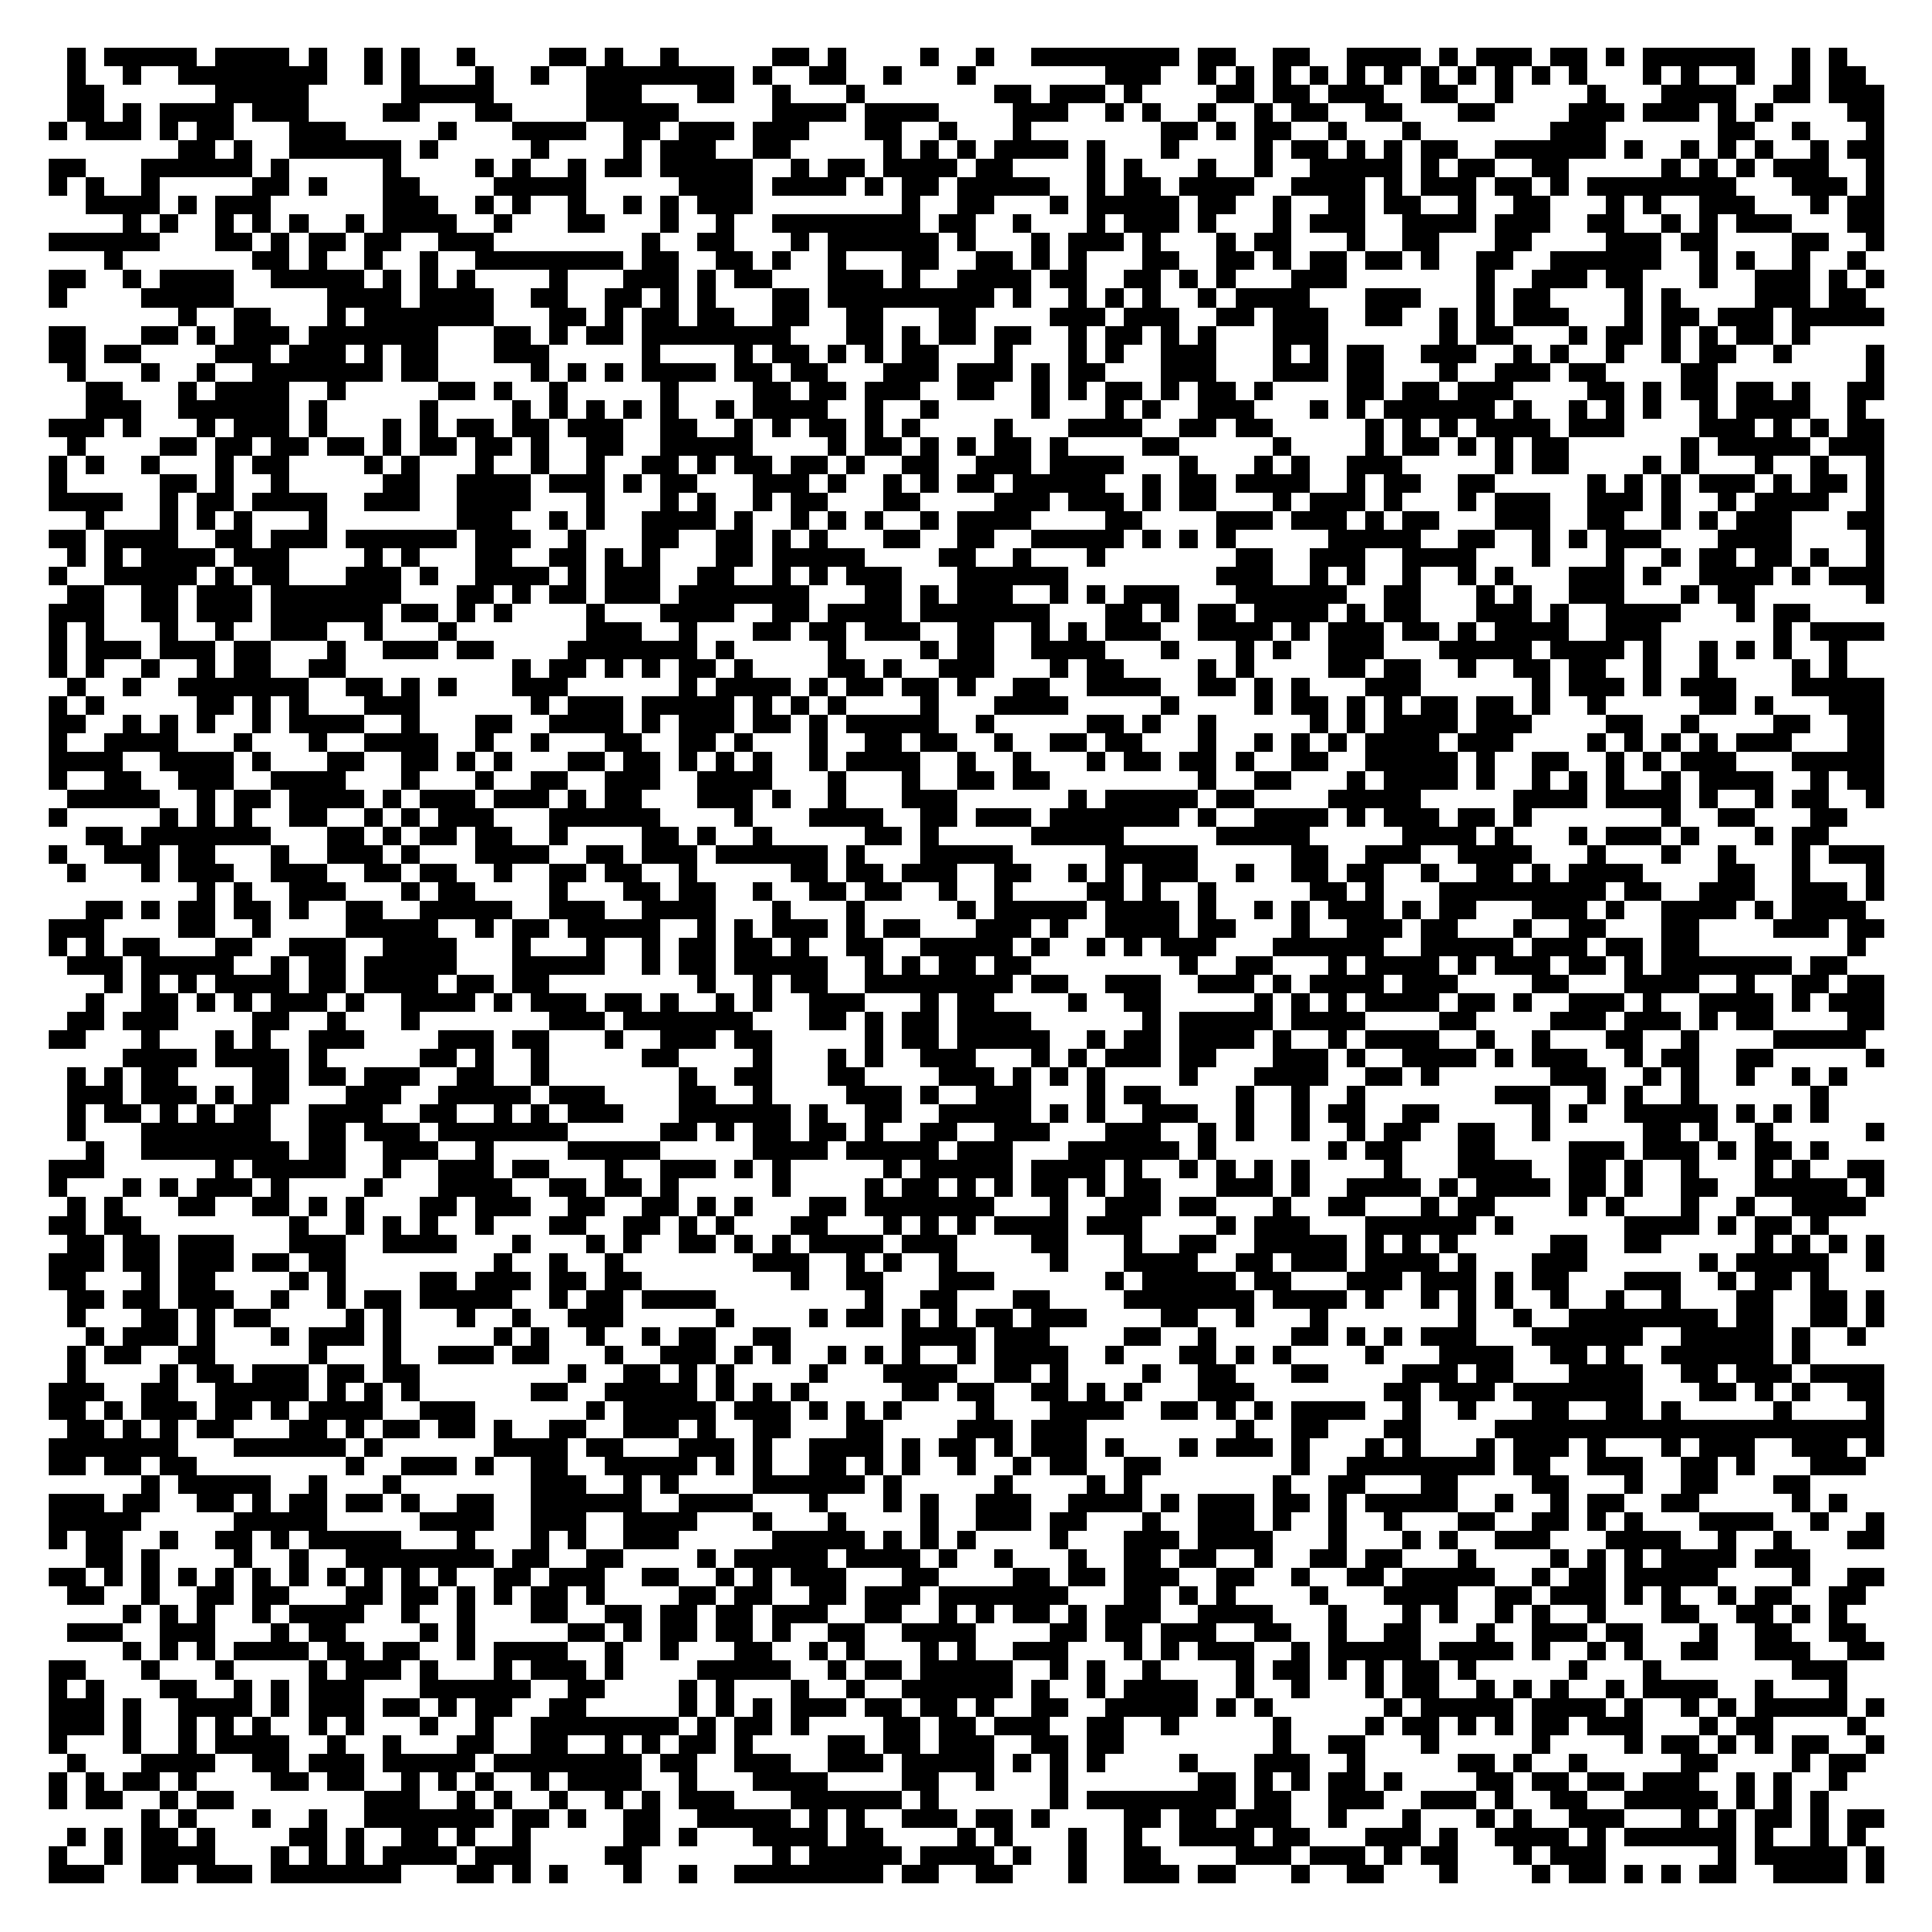
\includegraphics[width=0.7\textwidth]{mioni_matrika_dobra.png}
        \caption{}
        \label{fig: s2}
    \end{subfigure}
    \caption{Prikaz zaporedja bitov dobljenega iz naključnih števil.}
    \label{fig: m}
\end{figure}

\subsection{Dogodki z dvema elektronoma zbrani na detektorju CMS}
Podatke sestavlja $10^5$ dvo-elektronskih dogodkov invariantih mas 2-110 GeV zbranih na detektorju CMS \cite{CMS}.
Podatki vsebujejo energije $E$, gibalne količine $p$, transverzalne gibalne količine $p_t$, kote $\phi$ in $\eta$,
naboj $Q$ ($\pm1$) in invariantno maso obeh elektronov $M$ (slika \ref{fig: di_electron}).

Najprej si poglejmo zaporedje izmerjenih nabojev. Naboj pozitrona spremenimo v bit 1, naboj elektrona pa v bit 0.
Označimo naboj prvega nastalega elektrona s $Q^1_i$ in naboj drugega s $Q^2_i$. Poleg teh dveh zaporedij sem preizkusil še
zaporedji $\{Q_1^1, Q_2^1, \ldots, Q_N^2, Q_1^2, Q_2^2, \ldots, Q_N^2 \}$ in tudi
$\{Q_1^1, Q_1^2, Q_2^1, Q_2^2, \ldots, Q_N^1, Q_N^2 \}$. Iz spodnje tabele vidimo, da vsi testi potrdijo naključnost
bitnega zaporedja iz nabojev. Ostali dve zaporedji pa nista več tako dobro naključni.
Prvo zaporedje spodleti na spektralnem testu (spekter ima periodične značilnosti, ker smo ga sestavili iz dveh podobnih zaporedij),
drugo zaporedje pa spodleti kar na polovici testov. Razlog je v tem, da pari $Q_i^1, Q_i^2$ niso neodvisni. Lahko jih preštejemo in ugotovimo, da jih je
$\sim 43 \%$ enakih (00 ali 11) in da ostali niso enaki (10 ali 01), kar je v nasprotju s predpostavko
o enakomerni porazdelitvi podzaporedij.

\begin{table}[h!]
    \begin{center}
        \hspace*{-1.7cm}
        \begin{tabular}{cccccccccccccccc}
            \toprule
            {}                      & 1                       & 2                       & 3                       & 4                       & 5    & 6                       & 7                       & 8    & 9    & 10   & 11   & 12   & 13   & 14   & 15   \\
            \midrule
            \rowcolor{green!40}
            $p_{Q^1_i}$             & 0.08                    & 0.38                    & 0.08                    & 0.29                    & 0.58 & 0.18                    & 0.84                    & 0.22 & nan  & 0.10 & 0.38 & 0.16 & 0.07 & 0.53 & 0.43 \\
            \rowcolor{green!40}
            $p_{Q^2_i}$             & 0.18                    & 0.17                    & 0.64                    & 0.26                    & 0.33 & 0.06                    & 0.05                    & 0.41 & nan  & 0.74 & 0.65 & 0.10 & 0.11 & 0.45 & 0.69 \\
            $p_{Q^1_i\ldots Q^2_i}$ & 0.03                    & 0.09                    & 0.12                    & 0.29                    & 0.12 & \cellcolor{red!40} 0.00 & 0.62                    & 0.61 & nan  & 0.22 & 0.60 & 0.54 & 0.02 & 0.53 & 0.43 \\
            $p_{Q^1_i Q^2_i}$       & 0.03                    & 1.00                    & \cellcolor{red!40} 0.00 & \cellcolor{red!40} 0.00 & 0.70
                                    & \cellcolor{red!40} 0.00 & \cellcolor{red!40} 0.00 & \cellcolor{red!40} 0.00 & nan                     & 0.75 & 0.27                    & \cellcolor{red!40} 0.00 & 0.02 & 0.52 & 0.33                                    \\
            \bottomrule
        \end{tabular}
    \end{center}
    \caption{Statistični testi za zaporedje bitov iz izmerjenih nabojev.}
    \label{tab: 4}
\end{table}

\newpage

\begin{figure}[h!]
    \centering
    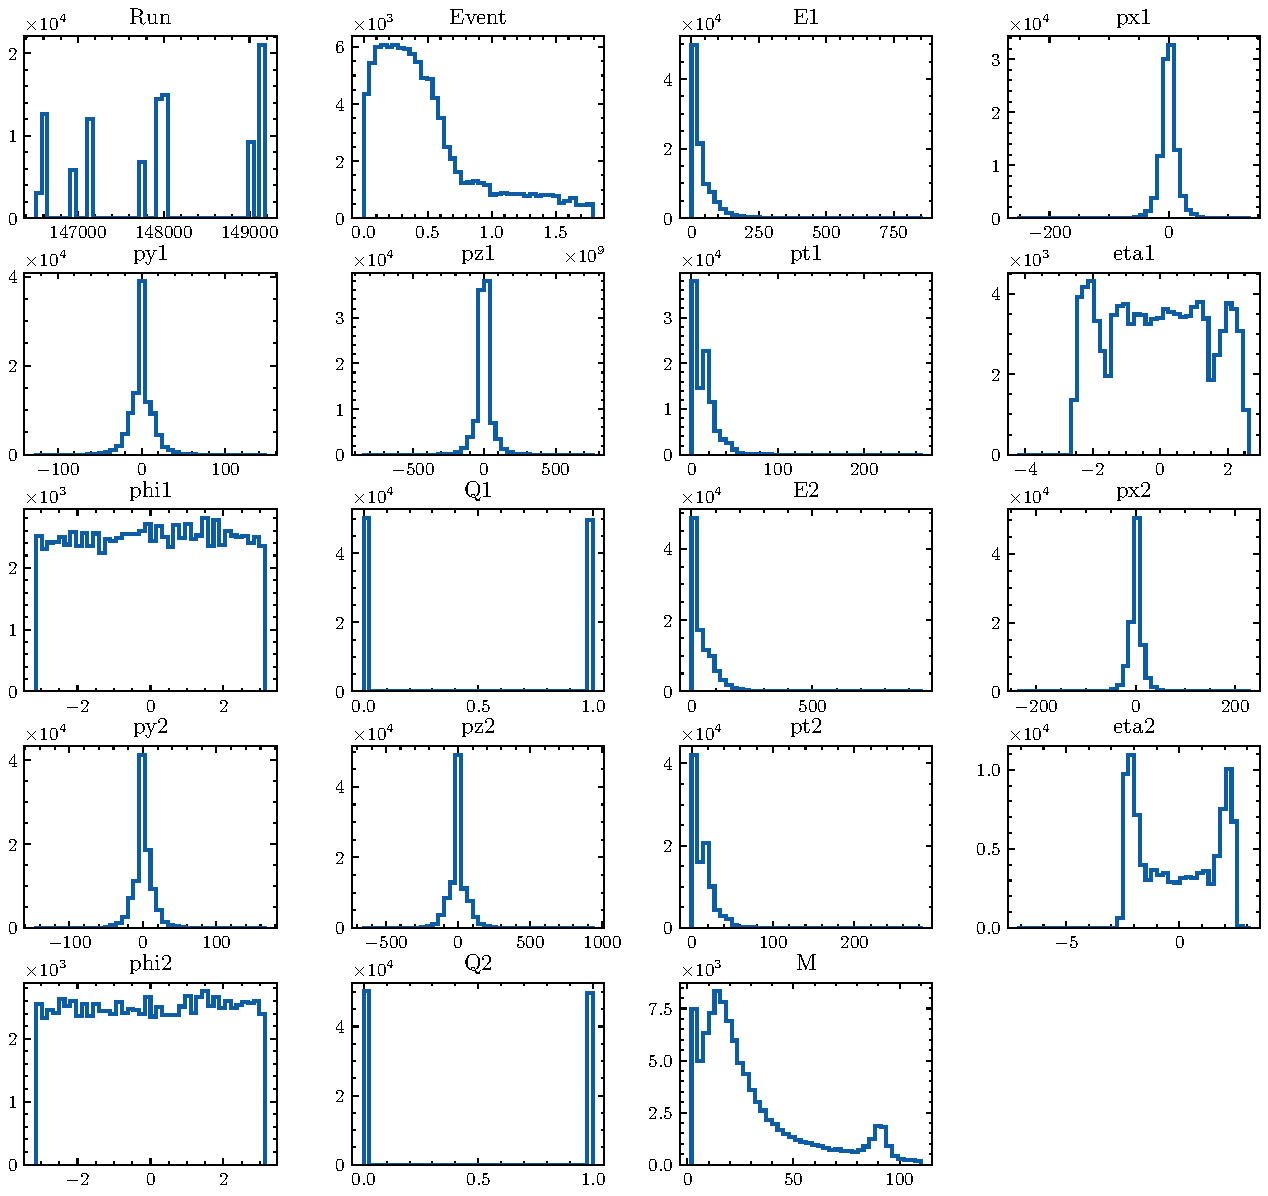
\includegraphics[width=0.95\textwidth]{dielectron_hists.pdf}
    \caption{Porazdelitve količin obeh elektronov (prvi dve nista pomembni).}
    \label{fig: di_electron}
\end{figure}

\noindent
Tokrat porazdelitve spremenljivk niso očitne in ne moremo uporabiti enakega postopka kot v prejšnjem primeru.
Nobena od porazdelitev tudi ni dovolj široka za uporabo Benfordovega zakona, zato bomo skonstruirali novo
porazdelitev kot zmnožek porazdelitev gibalnih količin
\begin{equation}
    f = \prod_{i=1}^N p_i \quad \text{kjer je} \quad p_i = \{p_{x1}, p_{y1}, p_{z1}, p_{x2}, p_{y2}, p_{z2}\} \>.
\end{equation}
Pričakujemo, da bo tako sestavljena porazdelitev lognormalna v limiti $N \rightarrow \infty$.
Slika \ref{fig: di_electron_lognorm} prikazuje zgoraj opisano množenje za vse različne $N$.
Vidimo, da pri povečevanju števila produktov res dobimo vse boljšo lognormalno porazdelitev.
Za generacijo naključnih števil uporabimo neceli del logaritma, kar nam da enakomerno porazdelitev.
Parametre $n_1$ (delež prvih enic), $\Delta n_1 = |n_1 - \log_{10} 2|$, $f_1$ (Fourierova komponenta porazdelitve pri
frekvenci 1) in rezultata $\chi^2$ ter KS prikazuje tabela \ref{tab: 5}.
Iz rezultatov vidimo, da so najbolj enakomerne porazdelitve za $N > 2$.
Izračunamo tudi vrednosti statističnih testov bitnega zaporedja (tabela \ref{tab: 6}), ki nam potrdijo domnevo o tem, da
so naključna samo števila iz porazdelitev pri $N > 2$.
% Če želimo, da bodo testi skladni s kriteriji predstavljenimi v tabeli \ref{tab: 5} moramo bitno
% zaporedje sestaviti po postopku \ref{eq: decide}. Razlog je v tem, da z rezanjem prvih nekaj bitov (ne upoštevamo cele številke)
% dodamo v zaporedje dodatno naključno komponento, kar ga naredi bolj naključnega.
% Rezultat je ta, da tudi test za $N=2$ postane uspešen.

\newpage

\begin{figure}[h!]
    \centering
    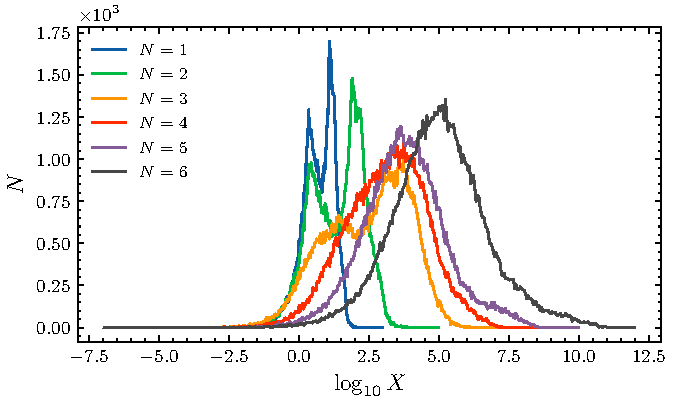
\includegraphics[width=0.8\textwidth]{dielectron_lognorm.pdf}
    \caption{Lognormalne porazdelitve kot produkt izmerjenih gibalnih količin.}
    \label{fig: di_electron_lognorm}
\end{figure}

\begin{table}[h!]
    \begin{center}
        \hspace*{-0.8cm}
        \begin{tabular}{cccccccc}
            \toprule
            {}    & $n_1$  & $\Delta n_1$ & $f_1$   & $\chi^2$ & $d$    & $p_{\chi^2}$ & $p_d$  \\
            \midrule
            $N=3$ & 0.3037 & 0.0027       & 0.00227 & 300.15   & 0.0040 & 0.7172       & 0.0877 \\
            $N=5$ & 0.3026 & 0.0016       & 0.00126 & 317.54   & 0.0045 & 0.4493       & 0.0334 \\
            $N=6$ & 0.3041 & 0.0031       & 0.00464 & 332.43   & 0.0036 & 0.2394       & 0.1394 \\
            $N=4$ & 0.3002 & 0.0008       & 0.00458 & 360.90   & 0.0020 & 0.0381       & 0.7945 \\
            $N=2$ & 0.3086 & 0.0076       & 0.00410 & 643.26   & 0.0159 & 0.0000       & 0.0000 \\
            $N=1$ & 0.3848 & 0.0837       & 0.00686 & 6523.96  & 0.1122 & 0.0000       & 0.0000 \\
            \bottomrule
        \end{tabular}
    \end{center}
    \caption{$\chi^2_*=377.41$ in $d_*=0.0051$ pri $\alpha=0.01$. Tabela je urejena glede na $\chi^2$ vrednost.}
    \label{tab: 5}
\end{table}

% \rowcolor{green!40}, \cellcolor{red!40}

\begin{table}[h!]
    \begin{center}
        \hspace*{-0.8cm}
        \begin{tabular}{cccccccccccccccc}
            \toprule
            {}    & 1                        & 2    & 3                        & 4    & 5    & 6    & 7    & 8    & 9    & 10   & 11                       & 12   & 13                       & 14   & 15   \\
            \midrule
            $p_1$ & \cellcolor{red!40}  0.00 & 0.06 & 0.47                     & 0.81 & 0.60 & 0.52 & 0.34 & 0.37 & 0.90 & 0.24 & \cellcolor{red!40}  0.00 & 0.08 & \cellcolor{red!40}  0.00 & 0.16 & 0.27 \\
            $p_2$ & \cellcolor{red!40}  0.00 & 0.51 & \cellcolor{red!40}  0.00 & 0.49 & 0.60 & 0.24 & 0.21 & 0.06 & 0.06 & 0.57 & 0.91                     & 0.79 & 0.00                     & 0.38 & 0.21 \\
            \rowcolor{green!40}
            $p_3$ & 0.29                     & 0.93 & 0.53                     & 0.77 & 0.86 & 0.44 & 0.56 & 0.13 & 0.67 & 0.02 & 0.42                     & 0.18 & 0.18                     & 0.34 & 0.42 \\
            \rowcolor{green!40}
            $p_4$ & 0.79                     & 0.35 & 0.69                     & 0.92 & 0.91 & 0.10 & 0.61 & 0.50 & 0.16 & 0.51 & 0.25                     & 0.05 & 0.82                     & 0.54 & 0.41 \\
            \rowcolor{green!40}
            $p_5$ & 0.86                     & 0.68 & 0.13                     & 0.90 & 0.18 & 0.03 & 0.20 & 0.89 & 0.99 & 0.25 & 0.57                     & 0.78 & 0.96                     & 0.66 & 0.49 \\
            \rowcolor{green!40}
            $p_6$ & 0.19                     & 0.72 & 0.87                     & 0.91 & 0.15 & 0.01 & 0.91 & 0.66 & 0.64 & 0.83 & 0.30                     & 0.07 & 0.24                     & 0.42 & 0.48 \\
            \bottomrule
        \end{tabular}
    \end{center}
    \caption{Rezultati statističnih testov za zaporedje bitov.}
    \label{tab: 6}
\end{table}

\newpage
\section{Naključna števila iz objav in komentarjev}
Poglejmo si ali lahko naključna števila generiramo še kako drugače. Kot vir podatkov bomo uporabili
Reddit (\emph{“the front page of the Internet”}). Razlog je v tem, da je Reddit precej bolj odprt za
zbiranje podatkov v primerjavi z drugimi platformami, kot sta Twitter in Facebook.
Za dostopanje do podatkov sem uporabil \cite{baumgartner2020pushshift}, ki omogoča 1 API klic na sekundo in
vsakič vrne 100 objav ali komentarjev.
Za generacijo naključnih števil bomo uporabili 600545 objav in 9661650 komentarjev, ki so bili narejeni na
različnih subredditih med 9. julijem in 8. avgustom 2021. Zbrani podatki vsebujejo:
ime avtorja, besedilo komentarja ali objave ter tudi naslov objave, čas objave (Unix timestamp format
natančen na eno sekundo), id objave in komentarja (uporabno za povezavo komentarja z objavo), število točk ter še
nekaj bolj tehničnih stvari, ki nas ne zanimajo.

\subsection{Časi objav in komentarjev}
Najprej si bomo ogledali številske podatke, potem pa se bomo lotili še tekstovnih podatkov.
Slika \ref{fig: times1} prikazuje porazdelitev časa komentarjev (za objave velja podobno). Na abscisni osi je prikazan
ura objave v našem poletnem času. V porazdelitvi nemudoma opazimo minimum, ki se zgodi okrog poldneva.
Razlog je v uporabnikih Reddita, ki so večinoma (več kot 50\%) Američani.
Premaknemo porazdelitev v nam najbližji ameriški časovni pas (slika \ref{fig: times2}) in ugotovimo, da do minimuma pride
okrog štirih zjutraj, kar je bolj skladno s pričakovanji. Vrh aktivnosti (v \emph{Eastern Daylight Time} času)
je torej ob 12, potem se začne počasi nižati vse do okrog polnoči, kjer začne strmo padati do zgodnjih
jutranjih ur. Preselimo se lahko v enega izmed bolj evropskih subredditov, kjer opazimo enako nihanje, ki je tokrat
v skladu z našim časom (slika \ref{fig: times3}).

\begin{figure}[h!]
    \centering
    \begin{subfigure}[b]{0.49\textwidth}
        \centering
        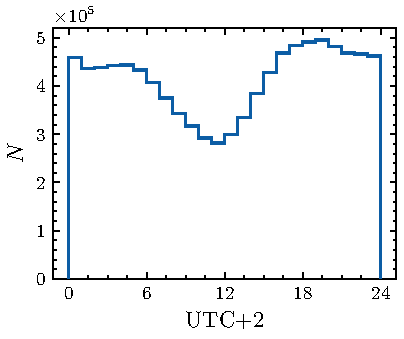
\includegraphics[width=0.83\textwidth]{reddit_times_dist_all.pdf}
        \caption{Porazdelitev časov objav.}
        \label{fig: times1}
    \end{subfigure}
    \hfill
    \begin{subfigure}[b]{0.49\textwidth}
        \centering
        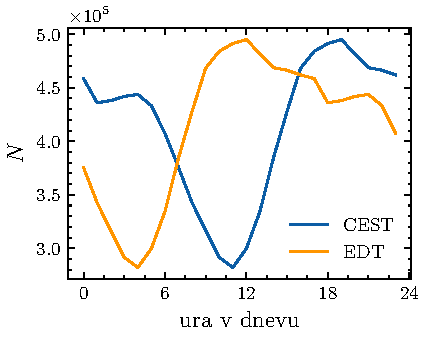
\includegraphics[width=0.83\textwidth]{reddit_timezones_dist.pdf}
        \caption{Različni časovni pasi.}
        \label{fig: times2}
    \end{subfigure}
    \hfill
    \begin{subfigure}[b]{0.49\textwidth}
        \centering
        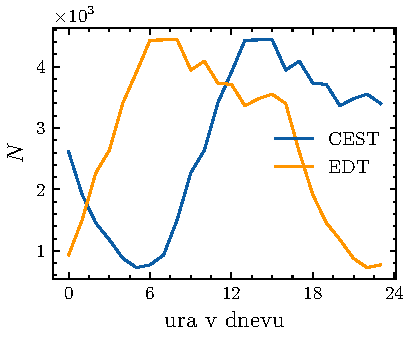
\includegraphics[width=0.83\textwidth]{reddit_eu_dist.pdf}
        \caption{Primerjava z evropsko demografiko.}
        \label{fig: times3}
    \end{subfigure}
    \caption{Časi komentarjev glede na časovni pas.}
    \label{fig: times}
\end{figure}

\newpage
Na žalost nam porazdelitev časov \ref{fig: times1} ne pomaga pri generaciji naključnih števil, ker
ni dovolj enakomerna. Namesto tega izračunamo razlike časov med objavo in njenimi komentarji $\Delta t$, kar je
prikazano na slikah \ref{fig: ptimes}. Prva slika prikazuje prelom v številu komentarjev.
V logaritemski skali se lepo vidita dve premici z različnima naklonoma
Do pojava pride zato, ker Redditov algoritem priotizira nove vsebino in začne skrivati objave, ki so stare več kot en dan.
Ker algoritem ni javen, tudi ne vemo kako se spreminja vidnost komentarjev pri ostalih časih.
Spodnji dve sliki prikazujeta porazdelitve razlik časov v intervalu do 10 minut ter v intervalu do enega dneva.
Vidimo, da največ komentarjev nastane takoj po objavi in da imajo časi potenčno odvisnost, ki
pa ne velja enako na celotnem območju (vmes se pojavi nekakšen plato).
Opazimo tudi, da so grafi precej podobni tistim iz \ref{fig: mu1}, ker gre pri obeh za podoben pojav.
Benfordov zakon za porazdelitev velja slabo (delež enic je samo 24\%), zato je ne moremo uporabiti direktno.

Za generacijo naključnih števil iz $\Delta t$ bomo spet uporabili medsebojno množenje bližnjih podatkov.
Rezultat je za $N$ množenj prikazan na sliki \ref{fig: ptimes4}. Vidimo, da nam več množenj vrne vse bolj
lognormalno porazdelitev za katero velja Benfordov zakon. Vzamemo logaritem necelega dela in dobimo enakomerno
porazdelitev, ki nam generira naključna števila. Naključnost je odvisna tudi od tega kako so bili na
začetku razvrščeni komentarji. Razvrstili bi jih lahko na več načinov (npr. glede na razne tekstovne
podatke), najbolj enostavno pa kar po številu točk, ki jih je prejel komentar.
Slika \ref{fig: rtimes} prikazuje odvisnosti že omenjenih statističnih količin od števila množenj $N$.
Iz slike vidimo, da dobimo dobro enakomerno porazdelitev že pri dveh množenjih.

Poglejmo si bolj podrobno statistiko testov pri $N=2$. Razdelimo besedilo tako, da dobimo 75 vzorcev, ki nam
vsak vrne po $10^6$ bitov. Za vsakega izmed vzorcev naredimo vseh 15 statističnih testov in zabeležimo $p$-vrednosti.
Če $H_0$ drži, pričakujemo, da bodo $p$-vrednosti porazdeljene po enakomerni porazdelitvi.
Rezultate, skupaj s $\chi^2$ vrednostmi za dobljeno enakomerno porazdelitev, prikazuje slika \ref{fig: pdist}.
Rezultati potrdijo, da sta za podatke \ref{fig: ptimes2} res dovolj že dve množenji

\vspace*{-0.5cm}

\begin{figure}[h!]
    \centering
    \begin{subfigure}[b]{0.49\textwidth}
        \centering
        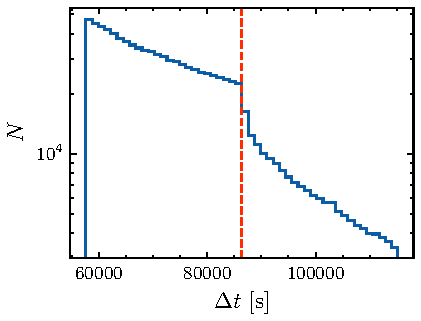
\includegraphics[width=0.83\textwidth]{reddit_post_activity_16h_to32h.pdf}
        \caption{Prelom v aktivnosti objave po enem dnevu.}
        \label{fig: ptimes1}
    \end{subfigure}
    \hfill
    \begin{subfigure}[b]{0.49\textwidth}
        \centering
        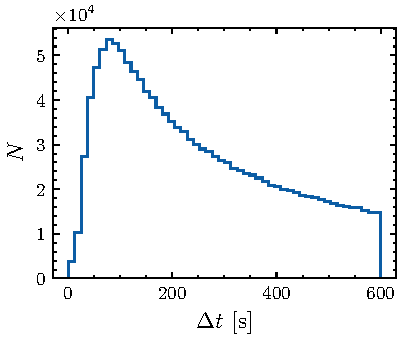
\includegraphics[width=0.8\textwidth]{reddit_post_activity_10min.pdf}
        \caption{Porazdelitev na intervalu $[0, 10]$ min.}
        \label{fig: ptimes2}
    \end{subfigure}
    \hfill
    \begin{subfigure}[b]{0.49\textwidth}
        \centering
        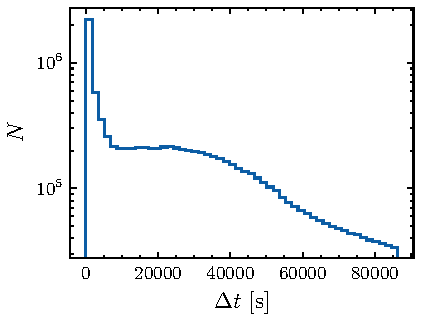
\includegraphics[width=0.83\textwidth]{reddit_post_activity_1day.pdf}
        \caption{Porazdelitev na intervalu $[0, 1]$ dan.}
        \label{fig: ptimes3}
    \end{subfigure}
    \hfill
    \begin{subfigure}[b]{0.49\textwidth}
        \centering
        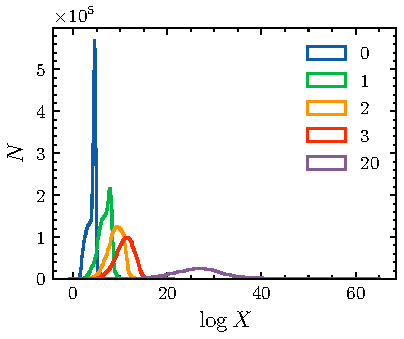
\includegraphics[width=0.8\textwidth]{reddit_lognorms.pdf}
        \caption{Lognormalne porazdelitve z množenjem.}
        \label{fig: ptimes4}
    \end{subfigure}
    \caption{Razlike časov med objavo in njenimi komentarji.}
    \label{fig: ptimes}
\end{figure}

\newpage

\begin{figure}[h!]
    \centering
    \begin{subfigure}[b]{0.49\textwidth}
        \centering
        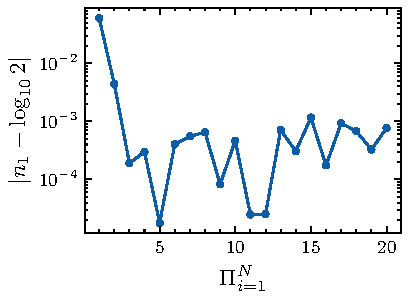
\includegraphics[width=0.9\textwidth]{reddit_times_n1.pdf}
        \caption{Razlika števila enic od napovedane.}
        \label{fig: rtimes1}
    \end{subfigure}
    \hfill
    \begin{subfigure}[b]{0.49\textwidth}
        \centering
        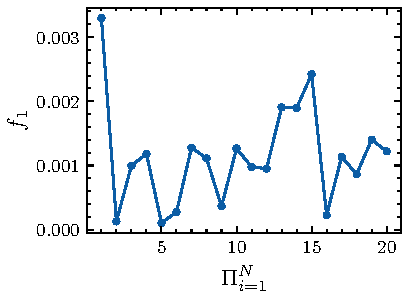
\includegraphics[width=0.9\textwidth]{reddit_times_f1.pdf}
        \caption{Fourierova komponenta.}
        \label{fig: rtimes2}
    \end{subfigure}
    \hfill
    \begin{subfigure}[b]{0.49\textwidth}
        \centering
        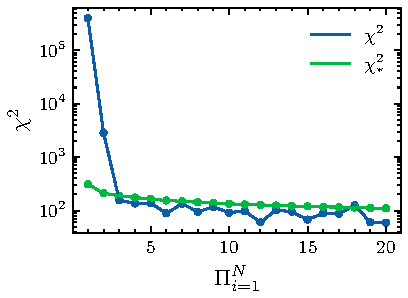
\includegraphics[width=0.9\textwidth]{reddit_times_chi2.pdf}
        \caption{$\chi^2$.}
        \label{fig: rtimes3}
    \end{subfigure}
    \hfill
    \begin{subfigure}[b]{0.49\textwidth}
        \centering
        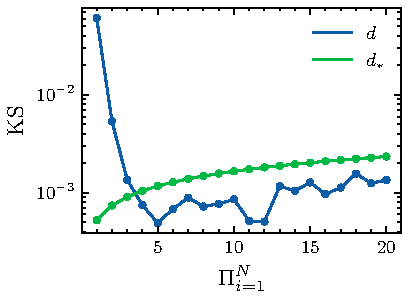
\includegraphics[width=0.9\textwidth]{reddit_times_ks.pdf}
        \caption{Kolomogorov-Smirnov.}
        \label{fig: rtimes4}
    \end{subfigure}
    \caption{Odvisnost opisanih količin od števila množenj (lognormalnosti porazdelitve).}
    \label{fig: rtimes}
\end{figure}

\begin{figure}[h!]
    \centering
    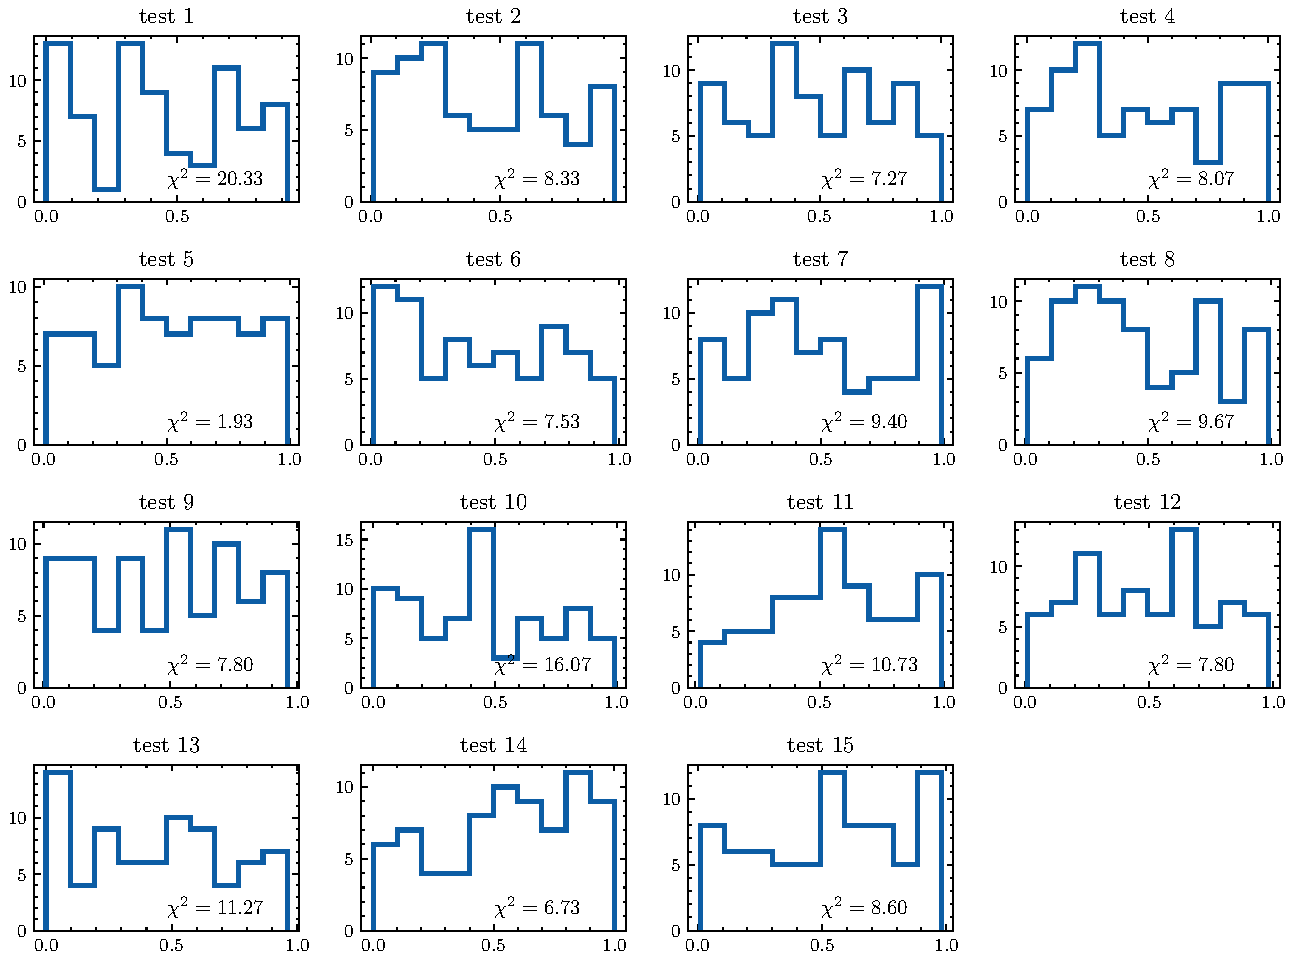
\includegraphics[width=0.8\textwidth]{p_test_dist.pdf}
    \caption{75 ponovitev NIST testov na različnih vzorcih po $10^6$ bitov pri $N=2$. $\chi^2_*=24.72$.}
    \label{fig: pdist}
\end{figure}

\newpage

\subsection{Naključna števila iz besedila}
Do zdaj smo vsa naključna števila sestavili iz numeričnih podatkov.
Največ informacije je v komentarjih in objavah seveda skrite v samem besedilu.
Poskusimo ali lahko naredimo naključna števila tudi iz takšnih tekstovnih podatkov.

Najprej preverimo s kakšnimi podatki imamo opravka. Na sliki \ref{fig: w} so prikazani histogrami 50 najbolj pogostih besed,
števila stavkov, znakov v komentarju ter števila znakov v vsakem stavku. Ocena števila stavkov je približna,
saj sem za definicijo stavka vzel del besedila, ki se začne z veliko začetnico in konča s piko.
Če komentar ne vsebuje nič od naštetega ga štejemo kot stavek.
Pri takem štetju se pojavi precej robnih problemov (npr. okrajšave), ki jih nisem upošteval.

Vse porazdelitve imajo dolg rep in predstavljajo potenčni zakon.  Iz takih porazdelitev ne moremo
direktno narediti naključnih števil lahko pa, enako kot v prejšnjem primeru, sestavimo lognormalno porazdelitev
z množenjem nekaj posameznih elementov v podatkih.
Ker smo to že naredili, si raje poglejmo način, ki uporabi znake besedila direktno.

\begin{figure}[h!]
    \centering
    \begin{subfigure}[b]{0.49\textwidth}
        \centering
        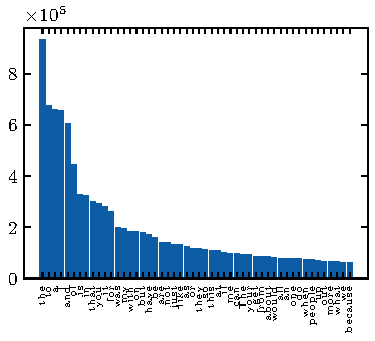
\includegraphics[width=0.84\textwidth]{word_count.pdf}
        \caption{Najbolj pogoste besede.}
        \label{fig: w1}
    \end{subfigure}
    \hfill
    \begin{subfigure}[b]{0.49\textwidth}
        \centering
        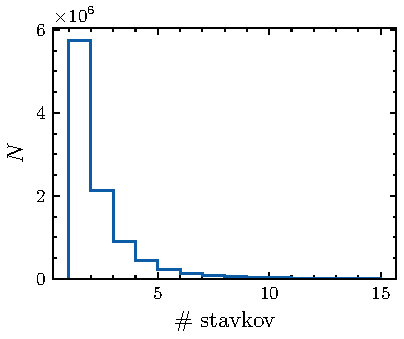
\includegraphics[width=0.9\textwidth]{sent_count.pdf}
        \caption{Število stavkov.}
        \label{fig: w2}
    \end{subfigure}
    \hfill
    \begin{subfigure}[b]{0.49\textwidth}
        \centering
        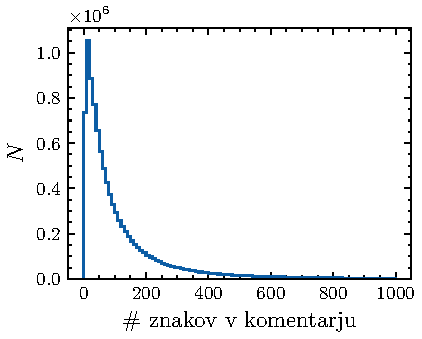
\includegraphics[width=0.9\textwidth]{char_comment_counts.pdf}
        \caption{Število znakov v komentarju.}
        \label{fig: w3}
    \end{subfigure}
    \hfill
    \begin{subfigure}[b]{0.49\textwidth}
        \centering
        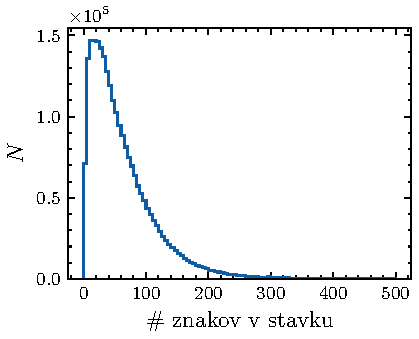
\includegraphics[width=0.9\textwidth]{sent_word_count.pdf}
        \caption{Število znakov v stavku.}
        \label{fig: w4}
    \end{subfigure}
    \caption{Nekaj karakterističnih porazdelitev iz besedila komentarjev.}
    \label{fig: w}
\end{figure}

\newpage
Znaki v besedilu so šifrirani v UTF-8 formatu \cite{wiki_utf8}. Različni znaki so predstavljani z enim do štirimi 8 bitnimi enotami.
Prvih 128 znakov je dolgih 1 byte in ustrezajo staremu ASCII formatu. Nekaj primerov:

\vspace*{-0.2cm}
\begin{figure}[h!]
    \centering
    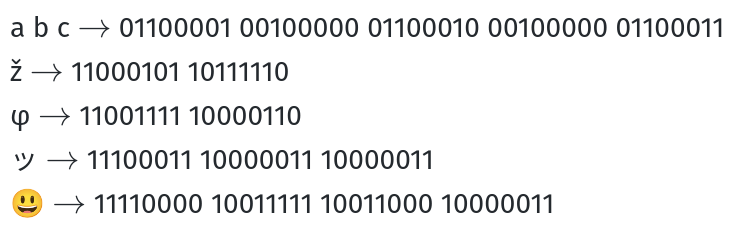
\includegraphics[width=0.55\textwidth]{utf8_primeri.png}
\end{figure}
\noindent
Ideja naključnega generatorja števil iz komentarjev in objav je naslednja (slika \ref{fig: text_rng}):
\begin{enumerate}
    \item Podatke dobimo preko API vmesnika (uporabimo poljubno HTTP requests knjižnico), ki nam vrne 100 objav/komentarjev na sekundo.
    \item Iz dobljenega besedila odstranimo presledke, nove vrstice in nekaj najbolj pogostih besed (ne več kot 100).
    \item Spremenimo znake besedila v UTF-8 format.
    \item Iz UTF-8 bitnih nizov vzamemo $i$-ti bit.
    \item Dobljeno bitno zaporedje premešamo, da razbijemo lokalno korelacijo v posameznem komentarju ali objavi. Uporabimo:
          \begin{equation*}
              \begin{aligned}
                   & \color{red}{ABCD} \color{black}{|} \color{ForestGreen}{EFGH} \color{black}{|}  \color{blue}{IJKL} \\
                   & \color{red}{A} \color{ForestGreen}{E} \color{blue}{I} \color{red}{B} \color{black}{|}
                  \color{ForestGreen}{F} \color{blue}{J} \color{red}{C} \color{ForestGreen}{G} \color{black}{|}
                  \color{blue}{K} \color{red}{D} \color{ForestGreen}{H} \color{blue}{L}                                \\
                   & \color{red}{A} \color{ForestGreen}{F} \color{blue}{K} \color{ForestGreen}{E} \color{black}{|}
                  \color{blue}{J} \color{red}{D} \color{blue}{I} \color{red}{C} \color{black}{|}
                  \color{ForestGreen}{H} \color{red}{B} \color{ForestGreen}{G} \color{blue}{L}                         \\
                   & \quad\>\>\> \vdots \quad\quad\>\>\>\> \vdots \quad\quad\>\>\> \vdots
              \end{aligned}
          \end{equation*}
          kjer vsaka črka predstavlja bit 0 ali 1 (primer prikazuje 12 bitov).
          Celoten postopek poskusi maksimizirati razdalje med začetnimi sosedi bitov.
          Zaporedje bitov najprej razdelimo v $m$ podskupin. Nove podskupine gradimo z zaporednim dodajanjem bitov iz
          naslednjih skupin. Prvi in zadnji bit se pri celem postopku ne spremenita. Postopek lahko ponovimo večkrat ter
          vsakič dobimo drugačno zaporedje.
    \item V premešanem zaporedju vzamemo $n$ zaporednih bitov ter iz njih tvorimo pozitivna neničelna cela števila.
    \item Dobljen vektor števil delimo s pozitivno neničelno konstanto $C$, da ne dobimo prevelikih števil. Vektor dimenzije $M$ spremenimo
          v matriko dimenzije $\lfloor \frac{M}{N} \rfloor \times N$ ter zmnožimo vse vrstice, kar nam vrne manjši vektor.
          Dobljena števila so po tem postopku porazdeljena lognormalno.
    \item Uporabimo ugotovitve Benfordovega zakona. Izračunamo neceli del logaritma, kar nam da enakomerno
          porazdelitev, ki jo preverimo s $\chi^2$ in KS testoma. Postopek lahko tukaj že končamo.
    \item Sledijo statistični testi za naključno zaporedje bitov. Dobljeno enakomerno porazdelitev pretvorimo nazaj v bitno zaporedje z odločitvenim drevesom ali
          pa z direktno pretvorbo pri kateri se moremo določiti do katerega bita bomo vzeli število.
    \item Naredimo vseh 15 NIST testov, ki nam vrnejo $p$-vrednosti glede na katere se odločimo ali je naključnost
          zaporedja sprejemljiva.
    \item Ponavljamo za različne prametre $\text{bit}_i, m, n, N$ dokler ni zaporedja bitov naključno.
\end{enumerate}

\newpage

\begin{figure}[h!]
    \centering
    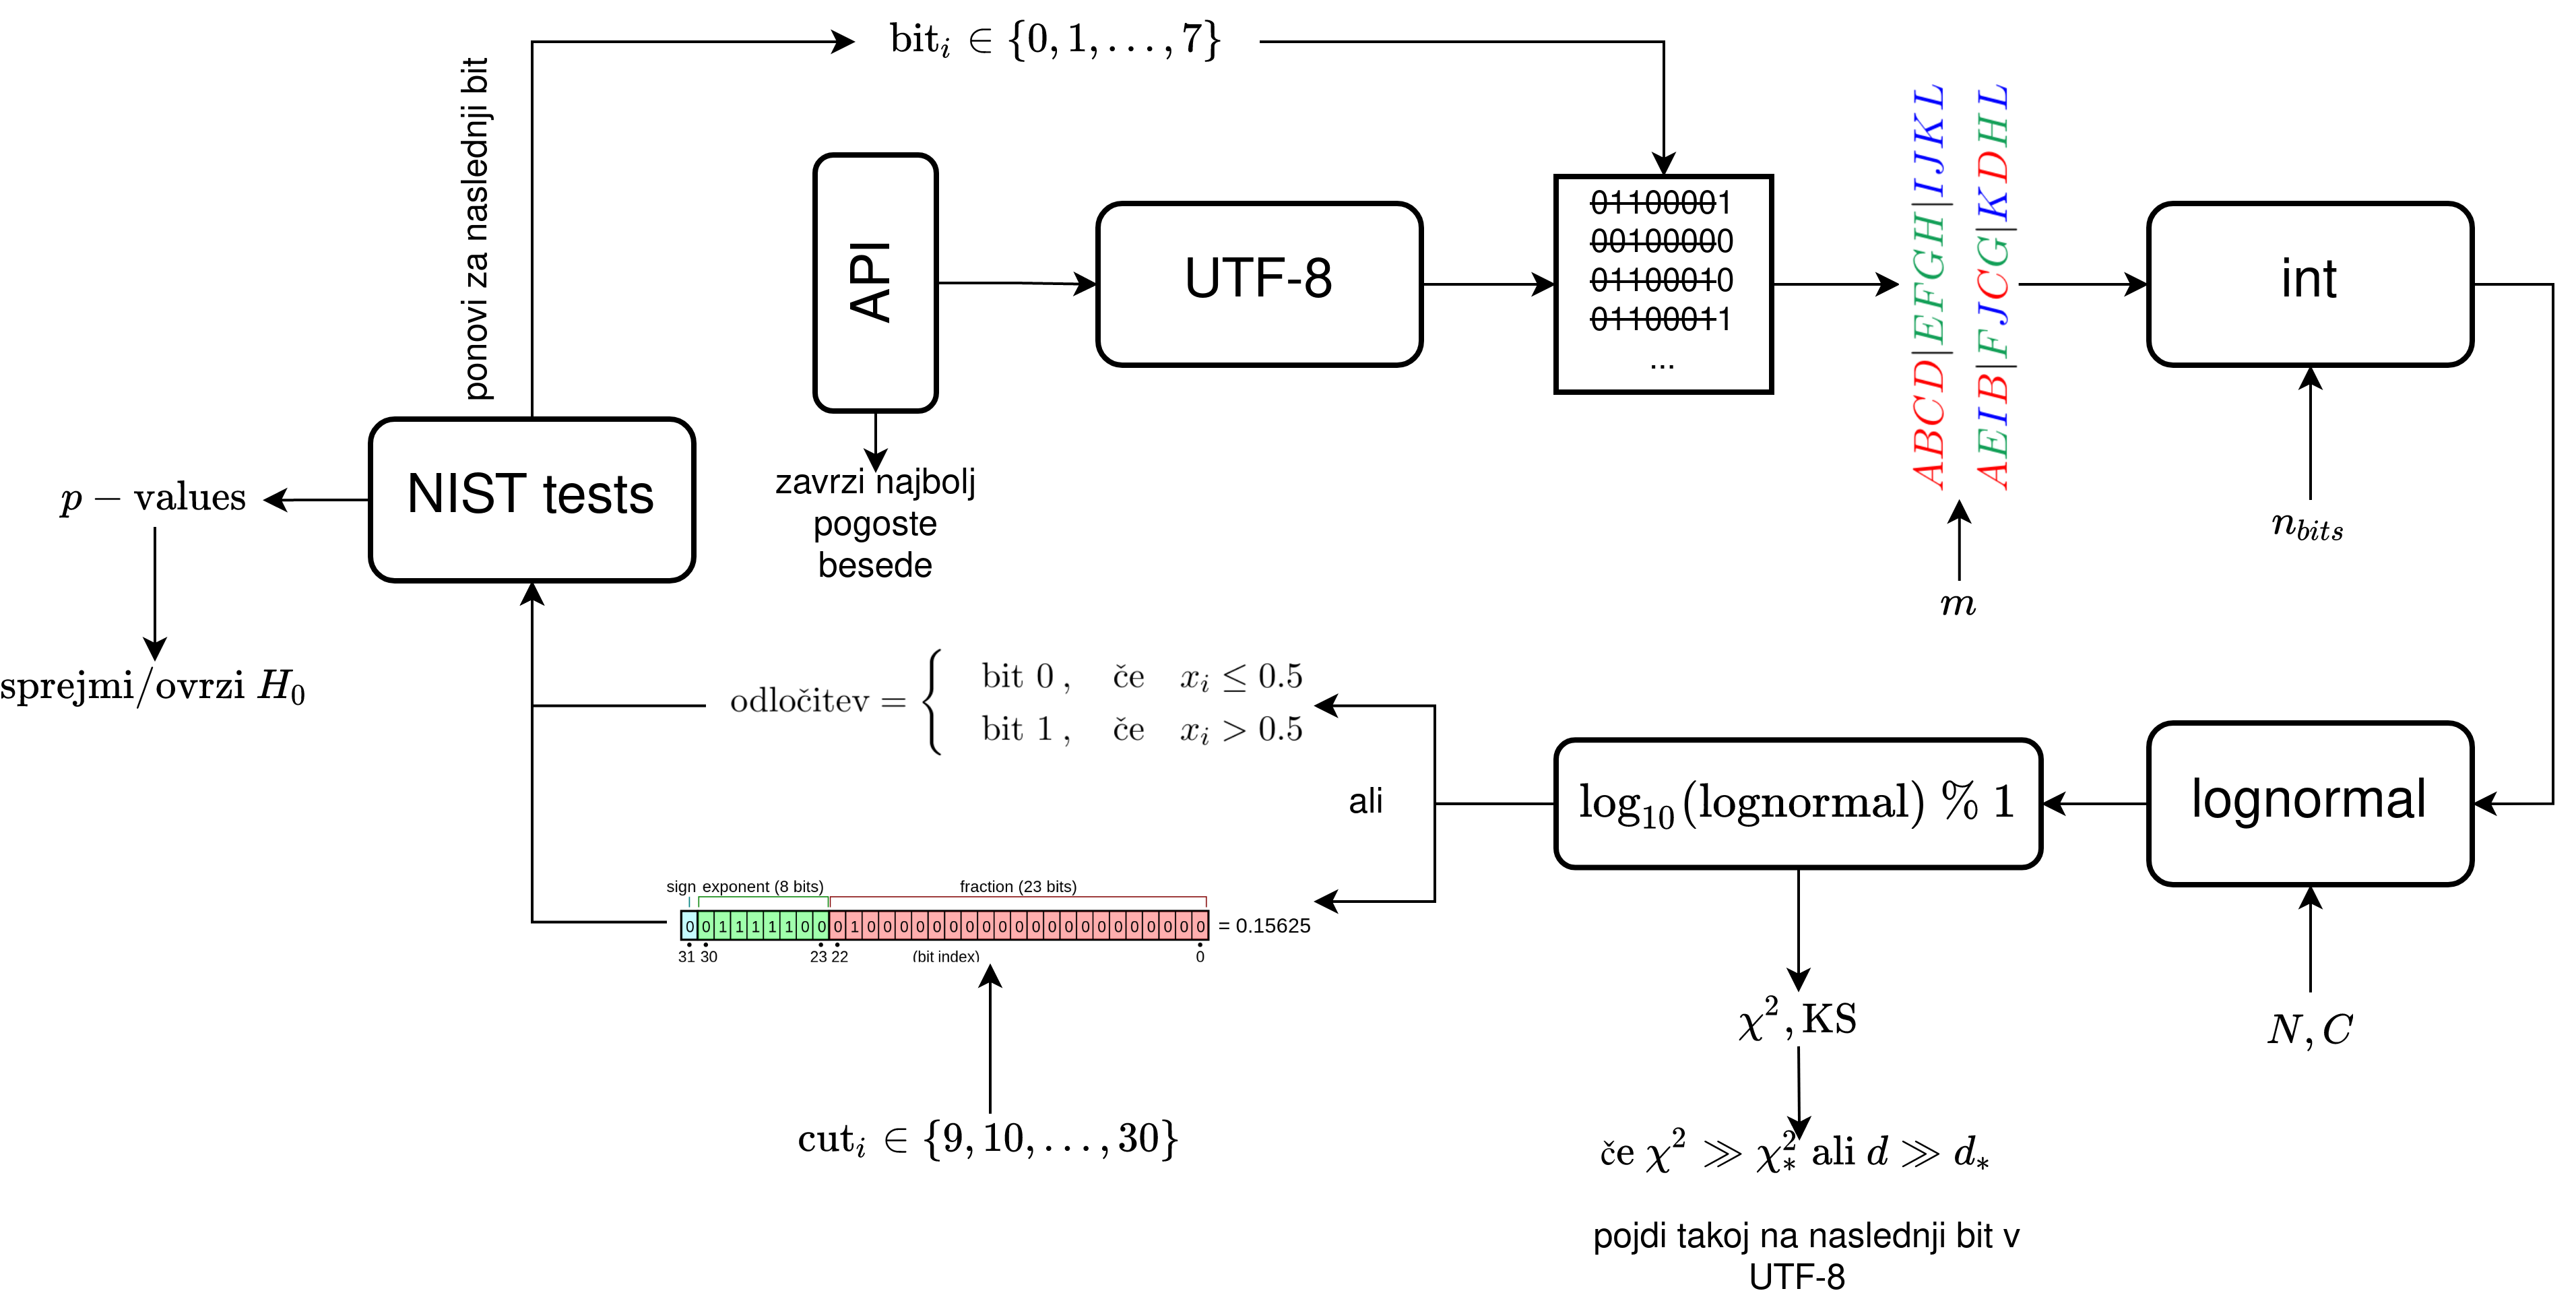
\includegraphics[width=1\textwidth]{text_rng_postopek.png}
    \caption{Postopek generacije in testiranja bitov dobljenih iz komentarjev.}
    \label{fig: text_rng}
\end{figure}

Postopek sem preveril na komentarjih, ki sem jih razdelil na $100$ vzorcev, ki vrnejo $2 \times 10^6$ bitov.
Rezultati statističnih testov za tri zadnje bite prikazuje slika \ref{fig: text_rng_results}.
Izkaže se, da prvi trije biti v UTF-8 niso naključni, naslednje dva sta vprašljivo naključna, rezultati
za ostale tri pa prikazuje spodnja slika. Za ostale parametre sem izbral: $m=16$ in samo eno mešanje, $n=8$,
$N=6$, $C=10^6$ ter $\text{cut}_i=9$.

\begin{figure}[h!]
    \centering
    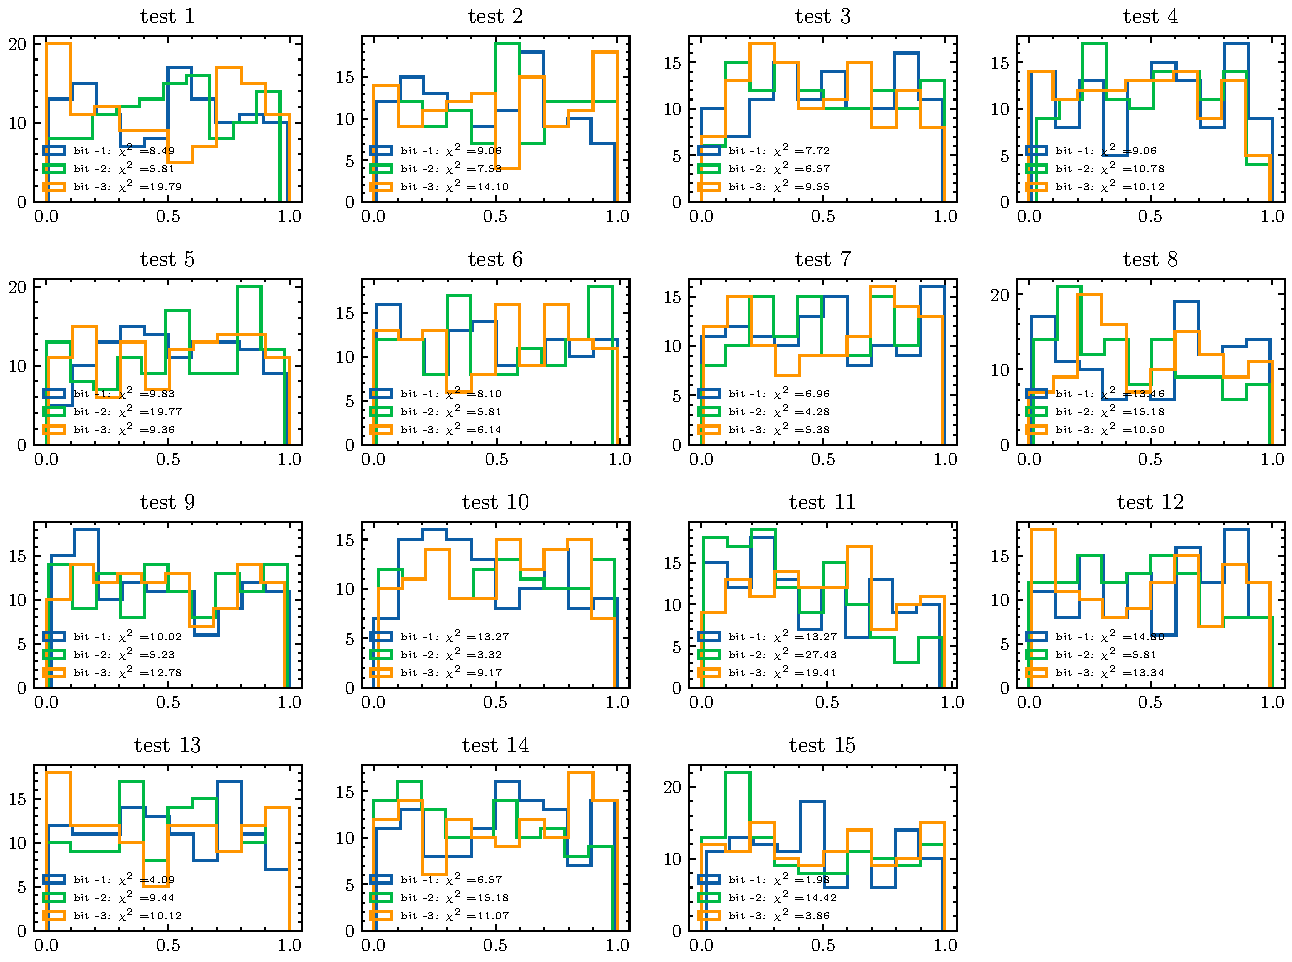
\includegraphics[width=0.98\textwidth]{text_rng_p_dists.pdf}
    \caption{Rezultati statističnih testov naključnosti za zadnje tri bite v UTF-8 formatu.}
    \label{fig: text_rng_results}
\end{figure}

\newpage
Naredimo še grobo oceno koliko naključnih bitov dobimo s tem postopkom na sekundo.
Izračun sem naredil za vzorec velikosti $10^6$ komentarjev. Vzorec je vseboval $1.305\times 10^9$ bitov (vsi znaki skupaj s presledki in novimi vrsticami), kar nam da
$\sim1300$ bitov na komentar. Postopek porabi $\sim 38$ začetnih bitov za en naključni bit. Upoštevamo limit
100 komentarjev na sekundo, kar nam da $\sim 3400$ naključnih bitov vsako sekundo (ali $\sim$ 150 z uporabo postopka \ref{eq: decide}).

\section{Zaključek}
Pri nalogi sem poskusil sestaviti generator naključnih števil iz konkretnih podatkov.
Generatorji, ki jih ponavadi uporabljamo niso naključni, saj za delovanje uporabljajo različne matematične
predpise, kar jih naredi predvidljive. Značilnost takih generatorjev je začetno seme ter neka končna perioda. S pravimi naključnimi
generatorji se lahko, na račun hitrosti same generacije števil, znebimo teh slabosti.

Naključna števila ne moremo dobiti direktno iz podatkov, ker ponavadi ne gre za enakomerno porazdelitev.
V ta namen sem uporabil Benfordov zakon iz katerega sledi, da so neceli deli logaritma števil porazdeljen enakomerno,
če seveda velja ta zakon. Izkaže se, da je porazdelitev za katero lepo velja Benfordov zakon lognormalna, ki
jo lahko dobimo z množenjem različnih količin, kar sledi iz centralnega limitnega izreka.
V nalogi sem pokazal, da Benfordov zakon velja dobro samo za dovolj široke lognormalne porazdelitve, kjer lahko
širino porazdelitve definiramo v Fourierovem frekvenčnem prostoru. Enakomernost tako dobljene
porazdelitve preverimo s testoma $\chi^2$ in testom Kolomogorov-Smirnova. Pojavi se tudi netrivialno vprašanje kako
vemo ali so dobljena števila zares naključna. V ta name sem uporabil NIST Statisical  Test  Suite, ki vsebuje
15 testov, ki preverjajo različne lastnosti naključnih zaporedij bitov.

Za generacijo naključnih števil sem najprej uporabil fizikalne podatke. Vzel sem meritve življenjskega
časa miona ter iz njih izluščil šum, ki je normalno porazdeljen. Enakomerno porazdelitev
sem iz standardne normalne genererial z inverzno Box-Mullerjevo transformacijo, kar se je izkazalo za precej uspešno.
Naslednji uporabljeni fizikalni podatki so bili dielektronski dogodki izmerjeni na detektorju CMS na LHC-ju.
Pokazal sem, da so posamezni predznaki nabojev elektronov porazdeljeni naključno. Iz ostalih podatkov (gibalnih količin)
pa sem generiral lognormalno porazdelitev ter pokazal, da je tudi tako dobljeno zaporedje števil naključno.

Iz fizikalnih podatkov sem na koncu prešel na podatke iz družbenih omrežij, kot so objave in komentarji.
Izkazalo se je, da časi objav niso enakomerno porazdeljeni, zato sem za generacijo naključnih števil uporabil
razlike časov med objavo in komentarjem, ki sem jih potem spremenil v lognormalno porazdelitev.
Najtežja je bila generacija naključnih števil iz samega besedila. Očitno je, da tekst komentarjev in
objav ni naključen. Predlagani algoritem vsebuje pretvorbo v UTF-8 format ter obravnavo samo zadnjih nekaj bitov in
njihovo mešanje, ki mu sledi znan postopek pretvorbe v lognormalno porazdelitev ter obravnavo logaritma
necelega dela. Postopek nam da, pri dobri izberi parametrov, sprejemljivo naključna števila glede na statistične teste.

\newpage

\selectlanguage{english}
\nocite{*}
\printbibliography[title={Literatura}]

\end{document}